\documentclass[11pt]{article}

\usepackage[margin=1in]{geometry}
\usepackage{amsmath,amssymb,amsthm,mathtools}
\usepackage{booktabs,tabularx,array}
\usepackage{graphicx}
\usepackage{caption}
\usepackage{float}
\usepackage{enumitem}
\usepackage{xcolor}
\usepackage{hyperref}
\usepackage[round]{natbib}
\usepackage{microtype}

\graphicspath{{figures/}}
\hypersetup{colorlinks=true,linkcolor=blue!50!black,citecolor=blue!50!black,urlcolor=blue!50!black}
\setlength{\parindent}{0em}
\setlength{\parskip}{0.45em}
\setlist[itemize]{leftmargin=1.3em,itemsep=0.12em,topsep=0.12em}
\setlist[enumerate]{leftmargin=1.45em,itemsep=0.12em,topsep=0.12em}
\setlength{\emergencystretch}{3em}
\allowdisplaybreaks

\newtheorem{proposition}{Proposition}
\newtheorem{lemma}{Lemma}
\newtheorem{corollary}{Corollary}
\theoremstyle{definition}
\newtheorem{definition}{Definition}
\newtheorem{remark}{Remark}
\newtheorem{assumption}{Assumption}

\newcommand{\dd}{\mathrm d}
\newcommand{\E}{\mathbb E}
\newcommand{\1}{\mathbf 1}
\newcommand{\Nset}{\mathcal N}
\newcommand{\Zset}{\mathcal Z}
\newcommand{\Sset}{\mathcal S}
\newcommand{\HH}{\mathcal H}
\newcommand{\Bcal}{\mathcal B}

\title{Intergenerational Housing Misallocation and Fertility}
\author{Tommaso De Santo}
\date{}

\begin{document}
\maketitle

\begin{abstract}
Children increase a household's demand for living space. Yet large rental
units are scarce, buying a family-sized home requires liquid wealth and access
to credit, and older households own much of the stock of large homes. I study
whether this allocation of housing raises the cost of having children for
young households. I first develop a simple overlapping-generations model in
which rental limits, down-payment constraints, and the retention decisions of
older owners determine who occupies family-sized housing. I then study the
same forces in a finite-life model with income risk, saving, tenure choice,
transaction costs, and bequests. The model distinguishes changes in family
size among current residents from changes in local births due to entry into the
housing market. The quantitative model suggests that restricted access to
family-sized housing matters for households deciding whether and when to have
children, and that home purchases and births are closely connected near the
end of the fertile years.
\end{abstract}

\subsection*{Status of this draft}

\begin{itemize}
\item I study a two-generation model that links access to family-sized housing
to the cost of children, derives the exact marginal-value gap between
constrained young buyers and old incumbents, defines equilibrium as a transition
between positive steady states, and gives explicit conditional existence
results.
\item I build a finite-life quantitative model with income risk, saving,
fertility, tenure choice, transaction costs, and bequests. The solution
produces a close connection between home purchases and births and
places a high value on additional space among constrained renters.
\item A grant for purchasing a family-sized home raises total births by
approximately 2.1 percent and the housing price by 0.90 percent. Combining the
grant with a tax on large homes raises total births by approximately 2.7
percent and lowers the housing price by 18.4 percent.
\item The analytical model characterizes mixed renter--owner positive steady
states, gives conditional existence results for a perfect-foresight transition,
and computes a horizon-stable transition approximation after one permanent
fertility-preference change. It also derives the exact local surplus from
reallocating housing across generations. The global ranking of policies that
change population remains a separate normative choice rather than an unstated
welfare criterion.
\item The quantitative model requires further evaluation, and further work is
needed on the calibration: the income-risk variance is provisional, and the
model overstates late-life homeownership. The
current version makes a one-time choice of completed fertility, so all children
arrive in a single cohort and age together. The main next extension is to add
sequential fertility, alongside strengthening the old-age downsizing margin,
reassessing identification, and further validating the entry response in the
policy exercises.
\item I do not report the project's empirical analysis in this note. Empirical
moments from the CPS, ACS, and PSID are used to discipline and evaluate the
quantitative model, but the construction of those moments and the reduced-form
evidence are left for a subsequent version.
\end{itemize}

\section{Introduction}
Children increase a household's demand for living space. Yet family-sized
housing is unevenly allocated across generations. Older households own much of
the stock of large homes, including after their children leave, while young
households deciding whether to have children are more likely to rent and have
limited liquid wealth. Large rental units are scarce, and buying a family-sized
home requires access to credit and a substantial down payment. This note asks
whether this allocation of housing across generations raises the cost of
having children and affects completed fertility---the number of children a
household has by the end of its fertile years---and local births.

The mechanism operates through access to space. When the rental market does
not offer sufficiently large units, a constrained renter values an additional
room above its posted rent. Ownership provides access to larger homes, but a
young household may be unable to finance the required down payment. At the
same time, transaction costs and tax rules can encourage older owners to remain
in large homes after their children leave. The resulting scarcity is therefore
not only a question of the aggregate housing stock. It also concerns who
occupies family-sized homes and whether those homes reach households making
fertility decisions.

I study this mechanism in two steps. A simple overlapping-generations model
shows how rental limits, financing constraints, and old-owner retention raise
the effective cost of accommodating children. I then embed these forces in a
finite-life model with income risk, saving, fertility, tenure choice,
transaction costs, and bequests. The quantitative model finds that many
renters making family-size decisions are constrained by the rental-size limit
and that home purchases and births are closely connected near the end of the
fertile years. I compare a grant for purchasing family-sized homes with a
package that combines the grant with a tax on large homes. Allowing entry and
population to respond, the grant raises total births by approximately 2.1
percent and the housing price by 0.90 percent; the package raises total births
by approximately 2.7 percent and lowers the price by 18.4 percent.

The distinction between birth timing and completed fertility is central to
this note. Quantitative lifecycle models show how economic conditions can
affect both when households have children and their completed fertility
\citep{sommerFertilityChoiceLife2016,doepkeBargainingBabiesTheory2019}.
Empirical work shows that house prices, housing wealth, and mortgage access
affect childbearing
\citep{lovenheimFamilyWealthShocks2013,dettlingHousePricesBirth2014,hacamoBabiesMortgageDeregulation2021}.
Recent studies also examine longer-run outcomes: \citet{dettlingKearneyModernMortgage2025}
present supplementary cohort correlations---positive for White women---between
cumulative FHA/VA lending and children ever born, and
\citet{vandoornikFazioRamadoraiSkrastinsHousingFertility2025} use random
variation in the timing of Brazilian housing-credit lotteries to estimate the
effects of earlier access on completed fertility among participants observed
after age 40. These
findings provide the empirical motivation for a quantitative lifecycle model
that separates changes in birth timing from changes in completed fertility and
can be used to evaluate housing policies in equilibrium.

% ==========================================================

% ==========================================================
\section{Analytical Model}
\label{sec:analytical_model}

This section studies two implications of housing access in a two-period
overlapping-generations economy.  A financing-constrained young buyer can value
family-sized space more than an old incumbent.  We also compare two positive
steady states and compute a terminally closed adjustment after a permanent
change in desired fertility.  In the numerical construction, that adjustment
generates house-price appreciation and taxable gains even though gains vanish
at either endpoint.  Appendix~\ref{app:olg_proofs} gives the household
solutions, transition results, and mixed-tenure construction.

\subsection{Environment}

\textbf{Households.}
At date $t$, the economy contains $Y_t$ young households and $O_t$ old
households.  A young household has income $y_i$, liquid wealth $b_i$, and
chooses total nondurable expenditure $c$, total housing $h$, completed
fertility $n$, saving $a'$, and tenure $m\in\{R,O\}$.  The pair $(y_i,b_i)$ is
drawn from a fixed distribution $F$ in each cohort; estates are warm-glow
expenditures rather than the source of the next cohort's $b_i$.

\textbf{Preferences.}
Each child uses $\chi>0$ units of goods and $\kappa>0$ units of housing.  Define
the parts of the household bundle available to the adults as
\begin{equation}
 x=c-\chi n>0,\qquad s=h-\kappa n>0.
 \label{eq:olg_usable_bundles}
\end{equation}
Young and old flow utilities are
\begin{align}
 u_t^Y(c,h,n)&=\log(c-\chi n)+\alpha\log(h-\kappa n)
 +\vartheta_t\log n,
 \label{eq:olg_young_utility}\\
 u^2(c^2,h^2,e)&=\log c^2+\gamma\log h^2+\omega_B\log e.
 \label{eq:olg_old_utility}
\end{align}
Here $e$ is a warm-glow estate.  Writing both $c$ and $h$ as gross choices makes
the two child requirements parallel: both reduce the household bundle left for
the adults.  Logarithmic utility keeps conditional demands and the response to
a binding housing limit in closed form; the mechanisms themselves enter through
access constraints and tax timing.

\textbf{Demography.}
A child born at $t$ produces $\nu>0$ young households at $t+1$, after survival
and household formation.  Thus
$Y_{t+1}=\nu\bar n_tY_t$ and $O_{t+1}=Y_t$, where $\bar n_t$ is average
fertility among the young.

\textbf{Housing and asset markets.}
The fixed housing stock is $\bar H$.  Rental units satisfy
$h\leq h_R^{\max}$, owner units satisfy $h\leq h_O^{\max}$, and
$h_R^{\max}<h_O^{\max}$.  The consumption good is the numeraire, and the
economy can trade it through a one-period bond with price $q\in(0,1)$ and gross
return $R_f=q^{-1}$; only the housing market must clear domestically.  The
property tax applies to every housing unit and is paid by the owner of record.
Owner-occupiers pay it directly; for a rental unit, the landlord is a
competitive intermediary that can trade the bond.  The intermediary buys one
unit for $P_t$ at the beginning of date $t$.  At the end of the period it
collects rent $r_t$, pays property tax $\tau^pP_t$, and carries a unit worth
$P_{t+1}$.  Since $R_f=q^{-1}$ is the gross return between the beginning and end
of the period, free entry imposes
\begin{equation}
 r_t+P_{t+1}=R_fP_t+\tau^pP_t
 \quad\Longleftrightarrow\quad
 r_t=(R_f+\tau^p)P_t-P_{t+1}.
 \label{eq:olg_rental_user_cost}
\end{equation}
Thus $r_t$ is paid in date-$(t+1)$ goods and $q\,r_t$ is its date-$t$ value.
Household budgets are written in beginning-of-period goods, so rent and the
property tax appear at their discounted values.  At a steady state,
$r=(R_f-1+\tau^p)P$.  Capital-gains taxation enters through owner-occupied
housing.  Rental intermediaries are not taxed on resale in the baseline, so
the gains tax does not enter \eqref{eq:olg_rental_user_cost}.  Appendix
\ref{app:olg_reallocation} gives the corresponding incidence calculation when
intermediaries are also taxed.

\textbf{Capital-gains taxation and home finance.}
Household capital gains are taxed only upon sale.  An old owner who bought one
unit at $P_{t-1}$ and sells it at $P_t$ pays the tax per unit
\begin{equation}
 \ell_t=\tau^g\max\{P_t-P_{t-1},0\},
 \label{eq:olg_prices}
\end{equation}
where $\tau^g$ is the capital-gains tax rate.  The owner pays tax only when
$P_t>P_{t-1}$.  If the owner keeps the house until death, appreciation accrued
during the owner's life is not taxed.  The estate's tax basis is reset to the
date-$(t+1)$ price, so an immediate estate sale realizes no taxable gain.  The
estate sale returns the unit to the fixed stock, and its proceeds enter the
warm-glow estate and leave the economy.  Selling while alive therefore
triggers a tax that retaining the unit avoids.  A young buyer finances the share
$\phi\in(0,1)$ and therefore posts $(1-\phi)P_th$ at purchase.

\subsection{Household problems}

Households take prices and transfers as given.  A renter buys housing services
and carries only financial wealth into old age.  An owner buys housing, posts a
down payment before receiving current income, and carries both mortgage debt
and the house into old age.

\textbf{Young renters.}
Conditional on renting, the young household solves
\begin{align}
 W_t^R(i)=\max_{c,h,n,a'}\;&u_t^Y(c,h,n)+\beta V_{t+1}^R(R_fa') \\
 \text{s.t.}\quad&
 c+a'+q\,r_th=y_i+b_i+T_t,\nonumber\\[-2pt]
 &h\leq h_R^{\max},\qquad a'\geq0.
 \label{eq:olg_young_renter}
\end{align}
The renter pays for housing services each period and enters old age with
financial wealth $R_fa'$.

\textbf{Young owners.}
Conditional on owning, the young household solves
\begin{align}
 W_t^O(i)=\max_{c,h,n,a'}\;&u_t^Y(c,h,n)+\beta V_{t+1}^O(a_{t+1},h) \nonumber\\
 \text{s.t.}\quad&
 c+a'+[(1-\phi)+q\tau^p]P_th=y_i+b_i+T_t,\nonumber\\[-2pt]
 &a_{t+1}=R_fa'-R_f\phi P_th,\qquad
 (1-\phi)P_th\leq b_i,\qquad h\leq h_O^{\max},\qquad a'\geq0.
 \label{eq:olg_young_owner}
\end{align}
The closing occurs before current income and tax rebates are available, and
unsecured borrowing is unavailable.  Thus only beginning-of-period liquid
wealth $b_i$ can satisfy the down payment.  The transfer $T_t$ is the date-$t$
present value of the equal per-household rebate of housing-tax revenue.

\textbf{Old households.}
An old household has financial wealth $a$.  An owner also carries housing $H$
from young age.  Renters and owners solve, respectively,
\begin{align}
 V_t^R(a)&=\max_{c^2,h^2,e}u^2(c^2,h^2,e),
 &c^2+qe+q\,r_th^2&=a+T_t,\quad 0<h^2\leq h_R^{\max},
 \label{eq:olg_old_renter}\\
 V_t^O(a,H)&=\max_{c^2,h^2,e}u^2(c^2,h^2,e),
 &c^2+qe+(q\,r_t-\ell_t)h^2&=a+(P_t-\ell_t)H+T_t,\nonumber\\[-2pt]
 &&0<h^2&\leq H,\quad e\geq P_{t+1}h^2.
 \label{eq:olg_old_owner}
\end{align}
The marginal cost of retaining a unit is therefore $q\,r_t-\ell_t$: selling
realizes the current tax, while retaining the unit avoids it.

\textbf{Tenure choice.}
Each household draws once an idiosyncratic preference $\xi_i$ for ownership,
independently of $(y_i,b_i)$, and observes it before choosing tenure.  It owns
when $W_t^O(i)+\xi_i\geq W_t^R(i)$.  Assume $\xi_i$ is logistic with
location $\bar\xi$ and scale $\sigma_\xi>0$, which gives the owner share
\begin{equation}
 \pi_t^O(i)=
 \frac{\exp\{[W_t^O(i)+\bar\xi]/\sigma_\xi\}}
 {\exp\{W_t^R(i)/\sigma_\xi\}+\exp\{[W_t^O(i)+\bar\xi]/\sigma_\xi\}}.
\label{eq:olg_owner_share}
\end{equation}
This cross-sectional preference heterogeneity makes aggregate tenure shares
smooth.  It does not enter the conditional renter or owner policies.

\subsection{Housing constraints and the cost of children}

Desired housing is the amount a household would choose without the rental or
down-payment limit.  The access constraint binds when this amount exceeds the
housing the household can obtain.  Its shadow value measures willingness to
pay for one more unit.

Fix a household $i$, a date $t$, and a tenure choice $m\in\{R,O\}$.  To obtain
closed forms, first suppose that saving and the household's old-age choices are
interior.  Let
$A=1+\gamma+\omega_B$ denote the sum of the old-age expenditure weights, and
let lifetime resources, valued at date $t$, be
\begin{equation}
 w_{it}=y_i+b_i+T_t+qT_{t+1}.
 \label{eq:olg_lifetime_objects}
\end{equation}
The current cost of housing depends on tenure:
\begin{equation}
 u_t^R=q\,r_t,\qquad u_t^O=q(r_t+\ell_{t+1}).
 \label{eq:olg_tenure_user_costs}
\end{equation}
A renter pays the present value of rent.  A buyer faces the same opportunity
cost and, if the unit is sold in old age, the anticipated gains tax.  Solving
the saving and old-age choices reduces the lifetime problem, up to a constant,
to
\begin{align}
 \max_{x,s,n}\quad &(1+\beta A)\log x+\alpha\log s+
 \vartheta_t\log n \nonumber\\
 \text{s.t.}\quad &(1+\beta A)x+u_t^m s+
 (\chi+\kappa u_t^m)n=w_{it}.
 \label{eq:olg_interior_lifetime_problem}
\end{align}
The term $\beta A$ summarizes old-age demand for consumption, housing, and the
estate.  With logarithmic utility, these three uses receive fixed expenditure
shares, so the same term appears in the reduced objective and budget.  The last
term in the budget gives the full resource cost of another child: $\chi$ units
of goods and $\kappa$ units of housing valued at the tenure-specific user cost.

Without a housing-access constraint, define
$D_t=1+\beta A+\alpha+\vartheta_t$.  The household then chooses usable goods,
usable housing, and fertility according to
\begin{equation}
 x^m=\frac{w_{it}}{D_t},\qquad
 s^m=\frac{\alpha w_{it}}{D_tu_t^m},\qquad
 n^m=\frac{\vartheta_t w_{it}}
 {D_t(\chi+\kappa u_t^m)}.
 \label{eq:olg_interior_policies}
\end{equation}
Gross choices are $c^m=x^m+\chi n^m$ and $h^m=s^m+\kappa n^m$.

Access may prevent the household from choosing this amount of housing.  A
renter cannot exceed the largest rental unit, while a buyer cannot exceed
either the largest owner unit or the amount supported by liquid wealth:
\begin{equation}
 \widehat h_{it}^R=h_R^{\max},\qquad
 \widehat h_{it}^O=\min\left\{h_O^{\max},
 \frac{b_i}{(1-\phi)P_t}\right\}.
 \label{eq:olg_effective_caps}
\end{equation}
If desired gross housing in \eqref{eq:olg_interior_policies} is below this limit, the
constraint is irrelevant.  Otherwise the household sets $h^m=\widehat h_{it}^m$,
and usable consumption and fertility solve
\begin{align}
 (1+\beta A)x^m+\chi n^m+u_t^m\widehat h_{it}^m&=w_{it},
 \label{eq:olg_binding_budget}\\
 \frac{\vartheta_t}{n^m}
 &=\frac{\chi}{x^m}
 +\frac{\alpha\kappa}{\widehat h_{it}^m-\kappa n^m}.
 \label{eq:olg_binding_fertility_foc}
\end{align}
The second equation prices the goods and housing taken from the adult bundle by
another child.  The appendix proves that these two equations have a unique
interior solution on the stated branch.

The value of relaxing the housing limit is the household's marginal value of
space minus its user cost:
\begin{equation}
 \zeta_{it}^m=
 \frac{\alpha x^m}{s^m}-u_t^m\geq0.
 \label{eq:olg_access_wedge}
\end{equation}
It is zero when housing is unconstrained and positive when an access limit
binds with a positive multiplier.  If the owner's physical size limit is slack
and the down-payment constraint binds, denote this financial component by
$\zeta_{it}^{O,F}$.
Combining the housing and fertility conditions gives
\begin{equation}
 \frac{\vartheta_t x^m}{n^m}
 =\chi+\kappa\bigl(u_t^m+\zeta_{it}^m\bigr).
 \label{eq:olg_full_price_child}
\end{equation}
Thus a binding access constraint raises the effective cost of a child by
$\kappa\zeta_{it}^m$.  This is the direct link between housing access and
fertility.
When the rental limit also binds in old age, committed old-age rent changes the
lifetime budget.  Appendix~\ref{app:olg_young_households} gives that branch.

\subsection{Positive steady states and transitions}

A permanent change in desired fertility moves the economy between two steady
states.  House prices and taxable gains are constant at either endpoint, but
can change during the transition.

At an arbitrary date, let $\bar n_t$, $\bar h_t^Y$, and $\bar h_t^O$ denote
average fertility, young housing, and old housing generated by current choices
and the old-state distribution.  At constant prices, transfers, and
preferences, write their stationary counterparts as functions of $(P,T;
\vartheta)$, and let $\bar h(P,T;\vartheta)=\bar h^Y(P,T;\vartheta)+
\bar h^O(P,T;\vartheta)$.  Market clearing and the government budget are
\begin{align}
 Y_t\bar h_t^Y+O_t\bar h_t^O&=\bar H,
 \label{eq:olg_housing_clearing}\\
 (Y_t+O_t)T_t&=q\tau^pP_t\bar H+\ell_tO_t\bar h_t^{\mathrm{sell}},
 \label{eq:olg_government}
\end{align}
where $\bar h_t^{\mathrm{sell}}$ is housing sold by old owners per old household, assigning
zero sales to renters.

\begin{proposition}[Steady-state accounting]
\label{prop:olg_steady_state}
Every positive steady state satisfies
\begin{align}
 \bar n(P^*,T^*;\vartheta)&=\frac{1}{\nu},
 &\ell^*&=0,\\
 T^*&=\frac{q\tau^pP^*}{2}\bar h(P^*,T^*;\vartheta),
 &Y^*=O^*&=\frac{\bar H}{\bar h(P^*,T^*;\vartheta)}.
 \label{eq:olg_steady_state_system}
\end{align}
Stationarity fixes average fertility at the replacement rate.  Prices,
transfers, tenure, individual fertility and housing, and the population scale
can nevertheless differ across steady states.
\end{proposition}

Stationarity requires replacement fertility; household choices and housing
clearing determine the price and population scale consistent with it.  Appendix
\ref{app:olg_steady_states} gives conditions for local determination.

Suppose $\vartheta_t$ rises permanently at date zero.  The economy starts from
the old steady state, so $S_0=(Y^0,Y^0,G^0,P^0)$ and $P_{-1}=P^0$.  Because the
old at date $t$ made their choices when young at $t-1$, the state must keep
track of their financial wealth, housing, and tenure.  Let $G_t$ denote this
distribution and write $S_t=(Y_t,O_t,G_t,P_{t-1})$.  Given $S_0$, a transition
equilibrium is a sequence of prices, transfers, household
choices, tenure shares, and distributions such that households optimize, the
cohort and distribution laws hold, housing clears, the government budget
balances at every date, and the sequence converges to the new steady state.
The two market conditions are
\begin{align}
 Y_t\bar h_t^Y+O_t\bar h_t^O&=\bar H,\\
 (Y_t+O_t)T_t&=q\tau^pP_t\bar H+\ell_tO_t\bar h_t^{\mathrm{sell}}.
 \label{eq:olg_transition_residuals}
\end{align}
The first equation clears the housing market.  The second rebates property-tax
revenue and the gains taxes paid by old sellers.

Figure~\ref{fig:olg_mixed_transition} uses a finite terminal closure.  From date
$J+1$ onward, prices and transfers equal their new steady-state values.  The
last young cohort faces those values in old age, but its purchase price $P_J$
remains its tax basis, so $\ell_{J+1}$ can be nonzero.  Its induced state is
recorded rather than imposed.  The computed path satisfies equilibrium through
date $J$ and approximates the remaining infinite sequence.
Appendix~\ref{app:olg_transitions} states conditions for a locally determined
solution to each finite system and shows that extending the terminal date
barely changes the reported path.  These checks do not establish existence or
uniqueness of the infinite-horizon transition.

One permanent shock is sufficient for several cohorts to realize gains.  The
cohort law can be iterated as
\begin{equation}
 Y_t=Y_0\prod_{s=0}^{t-1}\nu\bar n_s,
 \qquad O_t=Y_{t-1}.
 \label{eq:olg_iterated_cohorts}
\end{equation}
The first fertility response therefore changes the next young cohort, which
later becomes old and produces another cohort.  With a fixed housing stock,
this sequence can move prices for more than two dates.  Whenever
$P_s>P_{s-1}$, the old cohort selling at $s$ realizes
$\ell_s=\tau^g(P_s-P_{s-1})>0$.  The preference change is the only exogenous
shock in the construction below; the sign and duration of appreciation are
properties of its computed equilibrium path.

\begin{figure}[!htb]
\centering
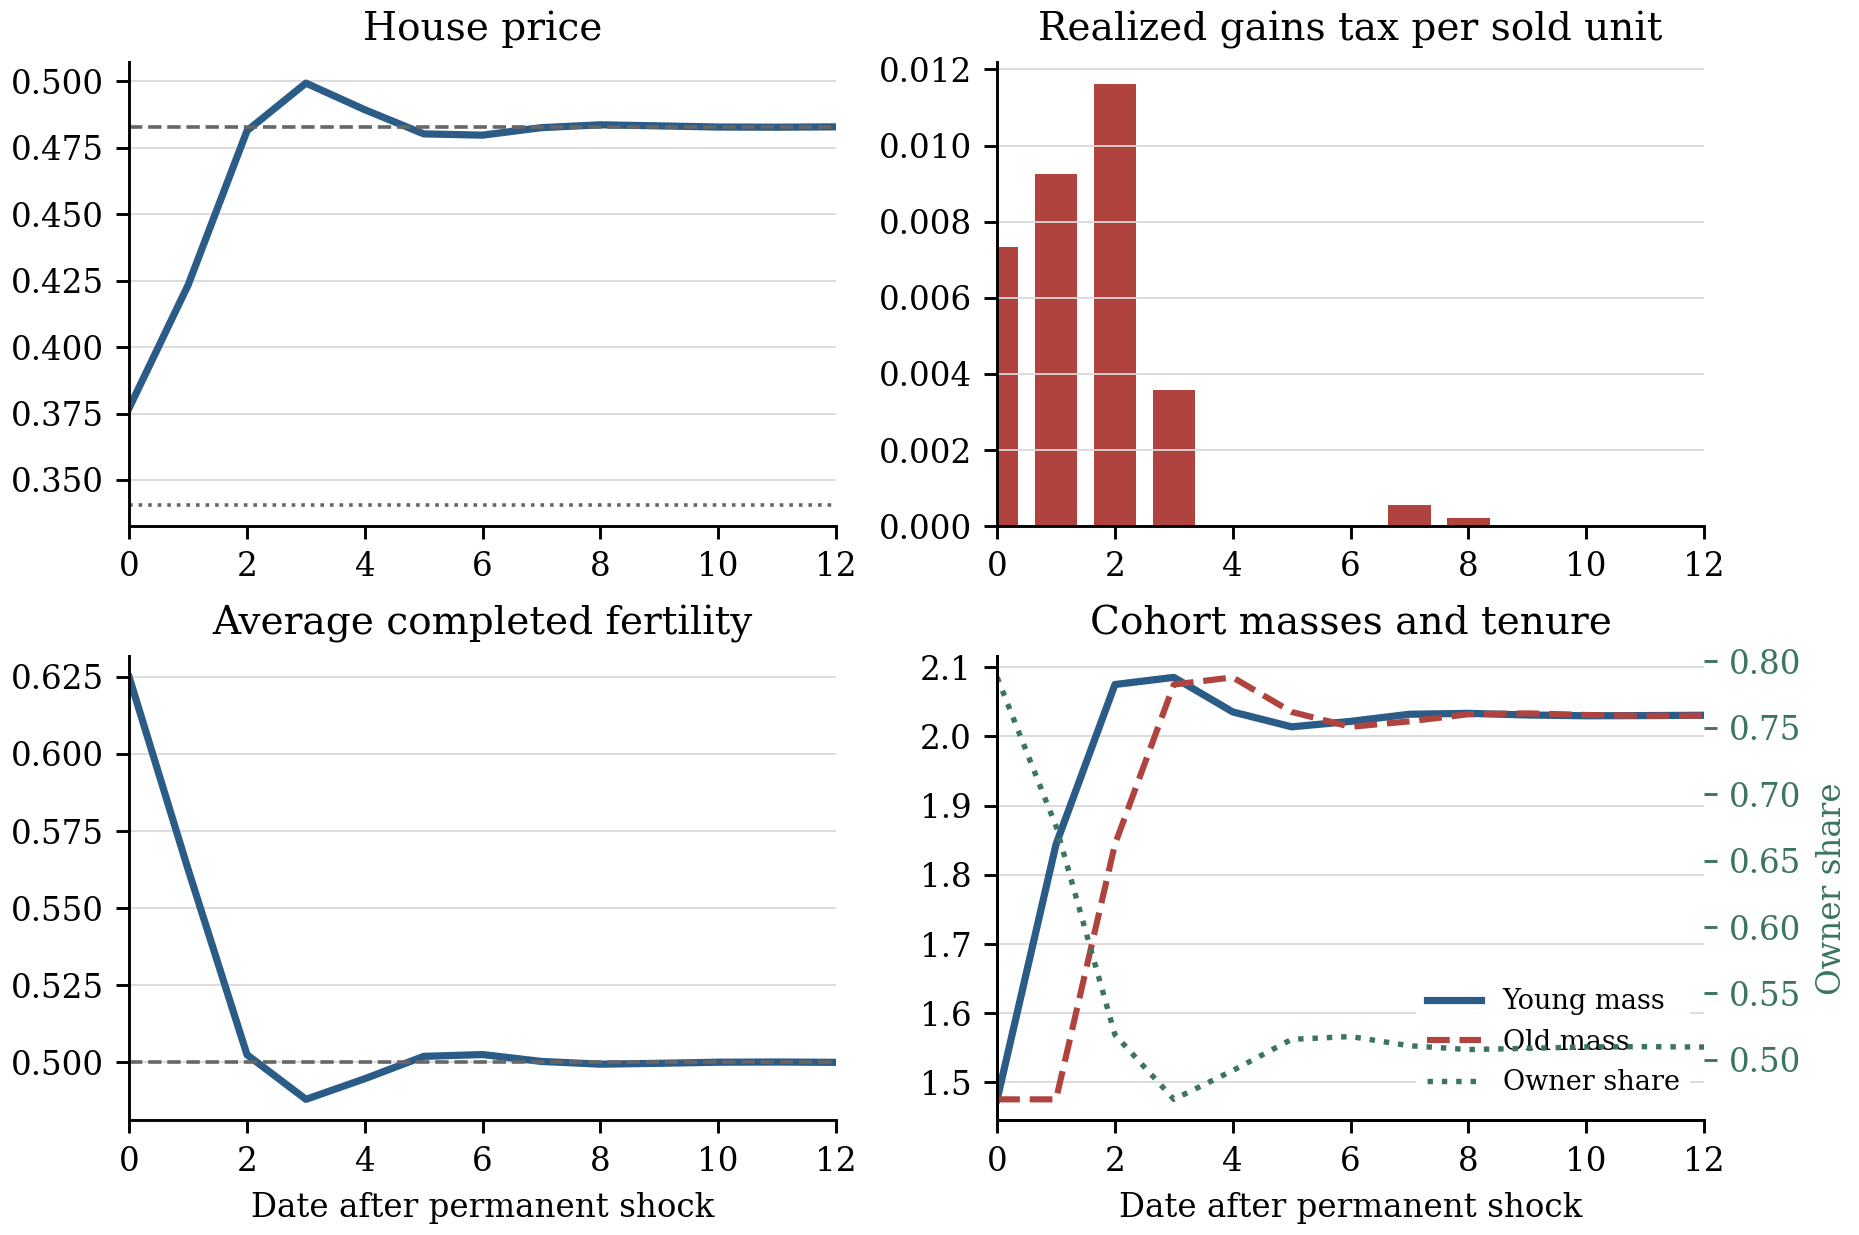
\includegraphics[width=0.55\textwidth]{figures/simplified_olg_mixed_tenure_transition.png}
\caption{Transition after a permanent increase in the fertility preference.
Lines mark steady-state prices and replacement fertility $1/\nu$.}
\label{fig:olg_mixed_transition}
\end{figure}

\subsection{Intergenerational reallocation and fertility}

Consider a marginal transfer of housing from an old incumbent to a young
owner, holding fertility, cohort sizes, tenure, prices, and other allocations
fixed.  The buyer's down-payment constraint binds; the other relevant choices
are interior.  Their marginal values of current housing services are
\begin{equation}
 MV_{it}^Y=q\,r_t+q\ell_{t+1}+\zeta_{it}^{O,F},
 \qquad
 MV_{jt}^O=q\,r_t-\ell_t.
 \label{eq:olg_marginal_values}
\end{equation}

The common term $q r_t$ is the value of housing services.  A sale costs the
incumbent $\ell_t$, the buyer anticipates $q\ell_{t+1}$, and the financing
constraint contributes $\zeta_{it}^{O,F}$.

Holding fertility, cohort sizes, and tenure fixed, call an allocation
\emph{conditionally locally efficient} if no small housing reallocation and
budget-balanced transfers can make all households alive at $t$ weakly better
off and one strictly better off.  Appendix~\ref{app:olg_reallocation} gives the
transfer scheme.

\begin{proposition}[Intergenerational reallocation]
\label{prop:olg_reallocation}
Under the conditions above and the two-date transfer ledger stated in
Appendix~\ref{app:olg_reallocation}, the marginal-value difference is
\begin{equation}
 MV_{it}^Y-MV_{jt}^O
 =\zeta_{it}^{O,F}+\ell_t+q\ell_{t+1}.
 \label{eq:olg_reallocation_surplus}
\end{equation}
Let $K_{ijt}\geq0$ be the marginal resource cost of transferring title and
occupancy.  Purchase and tax payments are transfers.  If
$MV_{it}^Y-MV_{jt}^O>K_{ijt}$, the allocation is not conditionally locally
efficient.
\end{proposition}

At a steady state the condition is $\zeta_i^{O,F}>K_{ij}$; the gains-tax terms
are transition-specific.  Thus the transfer improves the welfare of households
alive at $t$ when the value gap covers its resource cost.  The result does not
rank economies with different populations.

Let $\widehat h$ denote a binding housing limit.  Holding tenure, prices,
lifetime wealth, and the active set fixed, the interior old-age branch gives
\begin{equation}
 \frac{\dd n}{\dd\widehat h}\geq0
 \quad\Longleftrightarrow\quad
 \chi\leq
 \frac{(1+\beta A)\kappa(u_t^m+\zeta_{it}^m)^2}{\alpha u_t^m}.
\label{eq:olg_fertility_sign}
\end{equation}
Appendix~\ref{app:olg_fertility} derives this expression and the corresponding
capped-renter formula.
More accessible space raises fertility when children are sufficiently
space-intensive relative to their goods cost.  The same calculation gives
$\partial n/\partial w>0$ and $\partial n/\partial u_t^m<0$.  This is a
partial-equilibrium result; a funded policy also moves prices and transfers.


% ==========================================================
\section{Quantitative Lifecycle Model}
% ==========================================================
The quantitative model extends the analytical framework to a finite
lifecycle. It preserves the central mechanism: children raise the demand for
space, large rental units are scarce, ownership provides access to larger homes
but requires a down payment, and older households may retain family-sized homes
after their children leave. The model continues to have one housing market so
that the allocation of space across generations, rather than spatial sorting,
remains the central object.

The quantitative model adds the margins needed to evaluate this mechanism.
Households face income risk, save toward homeownership, and adjust their
housing over the lifecycle. Owner housing is a discrete ladder, while renters
choose space continuously up to a size limit. Households choose completed
fertility discretely during the fertile years; children subsequently age and
leave the household, while completed fertility continues to affect bequests.
Housing supply is upward sloping, and entry can change the scale of
the market in counterfactuals. Older households remain in their homes because
selling is costly and because housing enters the estate.\footnote{For now, the
quantitative exercises do not study capital-gains taxation or stepped-up
basis.}

\subsection{Lifecycle and Income}
Time is discrete. Households enter adult life at age $a=1$, retire after age
$J_R$, and die at the end of age $J$. Before retirement, labor income is the
product of a common wage, a deterministic age profile, and a persistent
idiosyncratic component:
\begin{equation}
y(a,z)=
\begin{cases}
(1-\tau_{\mathrm{pay}})w e_a z, & a\le J_R,\\
p^{\mathrm{ret}}, & a>J_R,
\end{cases}
\qquad
z'\sim \Pi^z(\cdot|z),
\label{eq:quant_income}
\end{equation}
Here, $e_a$ is the deterministic profile of expected household labor earnings
over the lifecycle, normalized to average one over working ages. The component
$z$ captures persistent differences in labor earnings across households of the
same age and is normalized to have invariant mean one. The common wage $w$
therefore sets the overall earnings scale, $e_a$ governs the common lifecycle
profile, and $z$ governs within-age earnings risk.

I specify $\log z$ as an annual AR(1), sample the implied process every four
years, and approximate it by a five-state Rouwenhorst chain. Annual persistence
is $0.960$ and the innovation standard deviation is $0.0645$, implying
four-year persistence of $0.85$ while preserving the stationary log-earnings
dispersion of the annual process.

\subsection{Preferences and Bequests}

Children raise minimum consumption and housing needs while they live at home.
Let $n_s$ be the number of dependent children and let $n$ denote completed fertility;
the two differ after children mature and leave. Household needs are
\begin{equation}
\begin{aligned}
\bar c(n,s)&=\bar c_0+\bar c_n n_s,\\
\bar h(n,s)&=\bar h_0
+\bar h_{\mathrm{jump}}\1\{n_s\ge1\}
+\bar h_n n_s.
\end{aligned}
\label{eq:quant_child_needs}
\end{equation}
The first child can create a discrete housing-space jump; additional dependent
children raise the required space linearly.

Preferences are CRRA over a Stone--Geary composite of consumption and usable
housing space. Write $h^R$ for rented space and $h$ for the owned housing stock;
only one can be positive. The owner service premium applies after household
needs are removed:
\begin{equation}
u(c,h^R,h;n,s)
=
\frac{
\left[
(c-\bar c(n,s))^{\alpha_c}
\mathbf h(h^R,h;n,s)^{1-\alpha_c}
\right]^{1-\sigma}
}{1-\sigma}
+\psi_{\mathrm{child}}n_s,
\label{eq:quant_flow_utility}
\end{equation}
where
\begin{equation}
\mathbf h(h^R,h;n,s)=
\begin{cases}
h^R-\bar h(n,s), & h=0,\\
\chi_O\big[h-\bar h(n,s)\big], & h>0,
\end{cases}
\qquad
\chi_O>0.
\label{eq:quant_housing_services}
\end{equation}
When $\chi_O>1$, ownership provides more utility from each unit of space left
after household needs are met. It does not change the physical number of rooms
required by children or the quantity of housing counted in market demand.

At death, households receive warm-glow bequest utility. The house passes to
the estate at market value: there is no forced sale, no transaction cost,
and no tax at death, so bequeathable wealth is $W^B=b+Ph$, liquid wealth
plus the gross value of any house held. For $\sigma\neq1$, bequest utility is
\begin{equation}
\Bcal(W^B,n)
=
\theta_0(1+\theta_n n)
\frac{
(\theta_1+\max\{W^B,0\})^{1-\sigma}-\theta_1^{1-\sigma}
}{1-\sigma}.
\label{eq:quant_bequest}
\end{equation}
For $\sigma=1$, the fraction is
$\log(\theta_1+\max\{W^B,0\})-\log\theta_1$.
The normalization sets $\Bcal(0,n)=0$, while the multiplicative term makes
completed fertility scale the marginal value of a positive estate.
Completed fertility can therefore affect saving even after children have
left the household.

\subsection{Housing, Finance, and Taxes}

There is one aggregate housing-services market. The rental user cost $r$ and
asset price $P$ satisfy
\begin{equation}
r=(q^{-1}-1+\delta+\tau^p)P.
\label{eq:quant_user_cost}
\end{equation}
Housing supply is upward sloping:
\begin{equation}
H^S(r)=\bar H\left(\frac{r}{\bar r}\right)^\eta.
\label{eq:quant_supply}
\end{equation}
Here $\bar r$ is the reference rental user cost, so housing supply equals
$\bar H$ at $r=\bar r$.
The fixed-stock compact model is the limiting case $\eta=0$ around the
benchmark stock. More generally, $\eta$ determines whether an increase in
housing demand appears mainly as a higher user cost or as additional housing.

Households either rent housing services or own one of $K$ discrete housing
sizes. The owned housing stock $h$ belongs to
\begin{equation}
\HH=\{0,H_1,\ldots,H_K\},
\label{eq:quant_housing_set}
\end{equation}
where $h=0$ denotes a renter and $h=H_k$ an owner of a house of size $H_k$,
ordered so that $H_1<\cdots<H_K$. Thus tenure is implicit in the housing
position rather than carried by a separate indicator. Renters choose $h^R$
continuously up to $\bar h^R$; owners choose from the discrete ladder. The
ladder is the quantitative version of the family-housing segmentation in
Section~\ref{sec:analytical_model}.

Renters choose $h^R\in[0,\bar h^R]$ and cannot borrow. Owners choose from the
discrete ladder and can borrow against the house. They pay maintenance and
property taxes through $(\delta+\tau^p)PH_k$.

At origination, a buyer can finance at most a share $\phi$ of house value, so the
required down payment is
\begin{equation}
    (1-\phi)PH_k.
\label{eq:quant_dp}
\end{equation}
Equivalently, adjusted liquid wealth immediately after purchase must satisfy
$\tilde b\ge-\phi PH_k$. End-of-period saving for every owner, whether a buyer
or an incumbent, faces the same debt floor:
\begin{equation}
b'\ge -\phi P H_k.
\label{eq:quant_ltv}
\end{equation}
The down payment governs entry into ownership, while the debt floor governs
resources after purchase. The distinction matters because a household can be
able to service an owned home and still lack the liquid wealth needed to buy it.

Housing adjustment is costly. A sale of an owned house $h>0$ incurs the
proportional transaction cost $\psi^s$, so net sale proceeds are
\begin{equation}
\Omega(h)
=(1-\psi^s)Ph.
\label{eq:quant_sale_proceeds}
\end{equation}
Transaction costs are the computed benchmark's disposal
friction.\footnote{Capital-gains taxation and stepped-up basis are left for
future quantitative work because incorporating them requires tracking each
owner's tax basis.}

\subsection{Fertility and Child Aging}

Fertility is chosen during the fertile window
\[
a\in\{A_f^{\mathrm{start}},\ldots,A_f^{\mathrm{end}}\}.
\]
A childless household chooses
\begin{equation}
n'\in\Nset=\{0,1,\ldots,\bar n\}.
\label{eq:quant_fertility_set}
\end{equation}
The option $n'=0$ means no birth in the current period. A positive choice fixes
completed fertility forever and moves its children into the first dependent
stage. A household that reaches the end of the fertile window
without a positive choice remains childless.

In the computation, $n\in\{0,1,2\}$ is a completed-fertility category rather than a
literal count of children.\footnote{The category $n=1$ represents families
with one or two children, while $n=2$ represents families with three or more.
The maintained scaling assigns two children to each unit of the index, so the
completed-fertility measure matched to the CPS is reported as $2\E[n]$.
Preferences, child needs, bequests, and demographic flows are evaluated in
index units.}

Let $s=0$ denote no dependent children and let $s=1,\ldots,S_c$ denote
dependent-child stages. After a positive fertility choice, the household enters
$s=1$. Children age stochastically through the stages according to $\Pi^c$.
While children are at home, $n_s=n$; after maturity, $n_s=0$. Completed
fertility still matters through bequest utility. All children therefore belong
to a single cohort and move through the child-age stages together. The model
does not yet allow sequential births or children of different ages; adding
sequential fertility is the main next extension of this block.

\subsection{Household Problem}

A household begins the period with liquid assets $b$, persistent earnings
component $z$, owned
housing $h$, age $a$, completed fertility $n$, and child stage $s$. If the
household is childless and in the fertile window, it first observes its
fertility taste shocks and chooses family size. Conditional on the current
family size, it observes its housing taste shocks and chooses the owned housing
position $h'$. It then chooses consumption $c$, end-of-period liquid assets
$b'$, and, if renting, current rental services $h^R$.

The choice $h'$ is made today and becomes the household's owned housing
position next period; $h'=0$ means that the household rents. Rental services
$h^R$, by contrast, are consumed only in the current period and therefore carry
no prime.

Before current housing transactions, the bond pays $b/q$. Liquid wealth after
changing housing from $h$ to $h'$ is
\begin{equation}
\tilde b(b,h,h')
=
\frac{b}{q}
+\1\{h>0,\ h'\neq h\}\Omega(h)
-\1\{h'>0,\ h'\neq h\}Ph'.
\label{eq:quant_adjusted_wealth}
\end{equation}
When $h'=h$, no house is traded. An owner who changes housing receives the net
sale proceeds $\Omega(h)$, while a household choosing a new owned house pays
$Ph'$. The renter and owner problems below are therefore evaluated at
$\tilde b(b,h,0)$ and $\tilde b(b,h,h')$, respectively.

Let the continuation value after earnings risk and child aging be
\begin{equation}
\bar V(b',z,h',a+1,n,s)
=
\E\left[
V(b',z',h',a+1,n,s')
\mid z,s,n
\right].
\label{eq:quant_continuation}
\end{equation}
The expectation is over next period's earnings component and child stage.
The terminal value is
\[
V(b,z,h,J+1,n,s)=\Bcal(b+Ph,n).
\]

Conditional on renting, the branch value is
\begin{equation}
\begin{aligned}
V^R(\tilde b,z,a,n,s)
=
\max_{c,h^R,b'}\quad
&u(c,h^R,0;n,s)+\beta \bar V(b',z,0,a+1,n,s)\\
\text{s.t.}\quad
&c+r h^R+b'=\tilde b+y(a,z),\\
&0\le h^R\le\bar h^R,\qquad b'\ge0.
\end{aligned}
\label{eq:quant_renter_problem}
\end{equation}
Conditional on choosing an owned house $h'>0$ after any adjustment, the branch
value is
\begin{equation}
\begin{aligned}
V^O(\tilde b,z,h',a,n,s)
=
\max_{c,b'}\quad
&u(c,0,h';n,s)+\beta \bar V(b',z,h',a+1,n,s)\\
\text{s.t.}\quad
&c+(\delta+\tau^p)Ph'+b'=\tilde b+y(a,z),\\
&b'\ge -\phi P h'.
\end{aligned}
\label{eq:quant_owner_problem}
\end{equation}
The debt floor is the same for a buyer and an incumbent. Renting offers a
continuous choice of space but no borrowing;
ownership offers the larger discrete menu and borrowing against the house, at
the cost of the initial down payment and future adjustment costs.
The housing-position value for a feasible $h'\in\HH$ is
\begin{equation}
\widetilde V^H(h'|b,z,h,a,n,s)
=
\begin{cases}
V^R(\tilde b(b,h,0),z,a,n,s), & h'=0,\\
V^O(\tilde b(b,h,h'),z,h',a,n,s), & h'\in\HH\setminus\{0\}.
\end{cases}
\label{eq:quant_housing_branch}
\end{equation}
The rent-or-own and owner-size choices have Type-I extreme-value shocks with
scale $\kappa_T$:
\begin{equation}
\pi^H(h'|b,z,h,a,n,s)
=
\frac{\exp\{\widetilde V^H(h'|b,z,h,a,n,s)/\kappa_T\}}
{\sum_{\hat h\in\HH}
\exp\{\widetilde V^H(\hat h|b,z,h,a,n,s)/\kappa_T\}},
\label{eq:quant_housing_probs}
\end{equation}
and the inclusive housing value is
\begin{equation}
V^H(b,z,h,a,n,s)
=
\kappa_T\log
\sum_{\hat h\in\HH}
\exp\{\widetilde V^H(\hat h|b,z,h,a,n,s)/\kappa_T\}.
\label{eq:quant_housing_iv}
\end{equation}
For a childless household in the fertile window, the value of fertility option
$n'$ is
\begin{equation}
\widetilde V^F(n'|b,z,h,a,0,0)
=
V^H(b,z,h,a,n',s(n')),
\qquad
s(n')=\1\{n'>0\}.
\label{eq:quant_fert_branch}
\end{equation}
With Type-I extreme-value shocks of scale $\kappa_F$,
\begin{equation}
\pi^F(n'|b,z,h,a,0,0)
=
\frac{\exp\{\widetilde V^F(n'|b,z,h,a,0,0)/\kappa_F\}}
{\sum_{\hat n\in\Nset}
\exp\{\widetilde V^F(\hat n|b,z,h,a,0,0)/\kappa_F\}}.
\label{eq:quant_fert_probs}
\end{equation}
The value before the fertility draw is the corresponding inclusive value:
\begin{equation}
V(b,z,h,a,0,0)
=
\kappa_F\log
\sum_{\hat n\in\Nset}
\exp\{\widetilde V^F(\hat n|b,z,h,a,0,0)/\kappa_F\}.
\label{eq:quant_fert_iv}
\end{equation}
Outside the fertile window, or after a positive fertility choice, this stage is
degenerate and $V(b,z,h,a,n,s)=V^H(b,z,h,a,n,s)$.
The family-size decision therefore incorporates the housing position chosen in
the same period. A birth can change current space and tenure immediately, not
only the household's continuation value.

\subsection{The Entry Problem}
\label{sec:quant_entry_problem}

At age 18, a potential household chooses whether to live in the modeled housing
market or in the outside economy. This choice is made before initial liquid
wealth and the persistent earnings component are realized. Conditional on entry, the household
draws $(b,z)$ from $G_E$ and begins adult life as a childless renter. Locally
born and outside-origin households draw from the same distribution $G_E$.

The value of entry is therefore
\[
W^E(r)=\int V(b,z,0,1,0,0;r)\,\dd G_E(b,z).
\]
The outside economy provides value $\bar W^E$. With Type-I extreme-value tastes
of scale $\kappa_E$, the fraction of potential households that enter is
\begin{equation}
q^E(r)
=
\frac{\exp\{W^E(r)/\kappa_E\}}
{\exp\{W^E(r)/\kappa_E\}+\exp\{\bar W^E/\kappa_E\}}.
\label{eq:quant_entry_probability}
\end{equation}
Housing costs affect entry through $W^E(r)$: a lower cost of living in the
modeled market raises the fraction of potential households that enter.

\subsection{Entry Equilibrium and Stationary Scale}
\label{sec:quant_entry_scale}

Let $g$ denote the beginning-of-period composition of adult households over
liquid wealth, the persistent earnings component, inherited owned housing, age, family size, and
child age, $(b,z,h,a,n,s)$, normalized to integrate to one. Let $S$ denote the
total adult population.

There are two sources of potential entrants. A fixed mass $M$ comes from the
outside economy. In addition, locally born children mature into potential
entrants. Let $B_0(g,r)$ denote the flow of mature locally born potential
entrants per unit of adult population. The total potential-entrant pool is
therefore $M+S B_0(g,r)$.

Let $E_0(g,r)$ denote the inflow of young adults required per unit of adult
population to reproduce the stationary composition $g$---equivalently, the
mass of age-one households in $g$. Stationarity requires the number who enter
to equal the number of young adults needed to replace the population:
\begin{equation}
q^E(r)\left[M+S B_0(g,r)\right]
=S E_0(g,r).
\label{eq:quant_scale}
\end{equation}
The left-hand side is the mass entering from the two potential-entrant pools;
the right-hand side is the inflow required to sustain an adult population of
size $S$.

For $M>0$, a finite positive adult population requires
$E_0(g,r)>q^E(r)B_0(g,r)$. Under this condition, rearranging
\eqref{eq:quant_scale} gives
\begin{equation}
S
=
\frac{q^E(r)M}{E_0(g,r)-q^E(r)B_0(g,r)}.
\label{eq:quant_scale_solution}
\end{equation}
Housing costs affect population scale through the entry probability $q^E(r)$,
while fertility affects scale through the future flow $B_0(g,r)$ of locally
born potential entrants.

The benchmark normalizes $S^\ast=1$.\footnote{Counterfactuals hold
$(M,\bar W^E,\kappa_E,G_E)$ fixed while entry, population scale, and the
housing-market equilibrium adjust.} Given the benchmark composition, I choose
$\bar W^E$ to deliver the benchmark entry probability $q^{E,\ast}$ and set
\[
M=\frac{E_0^\ast}{q^{E,\ast}}-B_0^\ast.
\]

\subsection{Stationary Equilibrium}
\label{sec:quant_stationary_equilibrium}

Throughout the equilibrium definition, $q$, $\delta$, and $\tau^p$ are fixed,
so $P=r/\rho$.

\begin{definition}[Stationary equilibrium]
A stationary equilibrium is a rental user cost and asset price $(r,P)$, value
functions and policies, housing and fertility choice probabilities, an entry
probability, stationary composition $g$, adult scale $S$, and aggregate housing
quantities such that:
\begin{enumerate}
\item households solve the branch problems
\eqref{eq:quant_renter_problem}--\eqref{eq:quant_owner_problem}, housing choice
is given by \eqref{eq:quant_housing_probs}, fertility choice is given by
\eqref{eq:quant_fert_probs}, and terminal utility is \eqref{eq:quant_bequest};
\item household choices and saving, together with earnings risk, child and adult
aging, death, and an inflow $E_0(g,r)\,\dd G_E(b,z)$ of age-one childless
renters, define a normalized transition operator $\mathcal T(g;r,S)$.
Stationarity requires
\begin{equation}
g=\mathcal T(g;r,S);
\label{eq:quant_stationary_distribution}
\end{equation}
\item entry and population scale satisfy \eqref{eq:quant_entry_probability}
and \eqref{eq:quant_scale}, with finite scale given by
\eqref{eq:quant_scale_solution};
\item let $\Pi^H(h'\mid b,z,h,a,n,s)$ and
$\widehat h^R(b,z,h,a,n,s)$ denote the housing-position probability and
expected rental space conditional on renting, respectively, after integrating
over the current family-size choice. Per-unit physical housing demand is
\begin{equation}
\begin{aligned}
\widehat H^D(g,r)
={}&
\int
\Bigg[
\Pi^H(0\mid b,z,h,a,n,s)\widehat h^R(b,z,h,a,n,s)\\
&\qquad
+\sum_{k=1}^K\Pi^H(H_k\mid b,z,h,a,n,s)H_k
\Bigg]\dd g(b,z,h,a,n,s).
\end{aligned}
\label{eq:quant_hd}
\end{equation}
\item the housing market clears in levels and the user-cost relation holds:
\begin{equation}
S\widehat H^D(g,r)=H^S(r),
\qquad
r=(q^{-1}-1+\delta+\tau^p)P;
\label{eq:quant_clearing}
\end{equation}
\item taxes, pensions, and any rebates satisfy the government accounting rule
specified for the calibration or counterfactual.
\end{enumerate}
\end{definition}

Equilibrium links family formation to housing through two margins. Children
change housing demand within a household, and, when locally born children feed
the future entrant pool, they also change the scale of the market. Housing
supply determines how much of either margin is absorbed by quantities rather
than by the user cost.

\subsection{Computation}
\label{sec:quant_computation}

One model period is four years. Period $j=0,\ldots,16$ begins at age
$18+4j$; the last interval covers ages 82--85. Retirement begins at 66, and
the last period in which a birth can occur begins at 42. Annual parameters are
converted before solution:
\[
q=(1+i_{\mathrm{ann}})^{-4},
\quad
\beta=\beta_{\mathrm{ann}}^4,
\quad
\delta=1-(1-\delta_{\mathrm{ann}})^4,
\quad
\tau^p=4\tau^p_{\mathrm{ann}}.
\]
The property-tax conversion is the undiscounted sum of four annual flow rates.
Income and consumption-flow quantities are expressed in four-year units;
housing remains in rooms.

The liquid-wealth grid spans $[-12,30]$, with a dense core on
$[-5,7]$ and a thinner upper tail beyond 15. The five-state Rouwenhorst
process has the following grid for the earnings component:
$z\in\{0.613,0.773,0.974,1.227,1.546\}$ and invariant weights
$\pi_z=(0.0625,0.25,0.375,0.25,0.0625)$. One dependent-child stage has an expected
duration of 18 years, giving a four-year maturity probability of $2/9$.
With deterministic $J$-period lives, the stationary normalized composition has age-one mass $E_0(g,r)=1/J$. The balanced pension equals payroll-tax
revenue per retiree in the stationary age distribution.

I solve the household problem by backward induction and obtain the stationary
distribution by forward iteration. The user cost adjusts until aggregate
housing demand equals supply.

\section{Calibration}
\label{sec:quant_calibration}

I organize the model parameters into two groups. The first consists of
parameters assigned from external evidence, measured directly in the data, or
fixed as maintained restrictions. The second consists of parameters estimated
internally by matching model moments to their empirical counterparts. I describe
the two groups in turn, explain which moments are particularly informative
about the internally estimated parameters, and then report the model's fit.

\subsection{Parameters Set Outside the Estimation}

I first describe the parameters assigned outside the estimation. Table~\ref{tab:quant_assigned}
summarizes their values and sources.

\paragraph{Demographics and preferences.}
A model period is four years. Households enter adult life at age 18, retire at
age 66, and live at most through age 85. Survival is certain before retirement
and thereafter follows four-year probabilities constructed from the combined
male and female survivor counts in the 2023 Social Security period life table.
Dependent children remain in the household for an expected 18 years, implying
a maturity probability of $2/9$ per period. I set risk aversion to $\sigma=2$.

\paragraph{Housing finance and transaction costs.}
Following \citet{greaneyDynamicUrbanEconomics2025}, I set the annual real
return on liquid wealth to $i_{\mathrm{ann}}=0.02$, annual housing depreciation
to $\delta_{\mathrm{ann}}=0.011$, the proportional selling cost to
$\psi^s=0.06$, and the labor-income tax rate to
$\tau_{\mathrm{pay}}=0.179$. The return is based on the average ten-year real
interest rate, depreciation combines BEA residential-structure depreciation
with an adjustment for the land share of house values, and the tax rate comes
from OECD data. I set the annual property-tax rate to
$\tau^p_{\mathrm{ann}}=0.01$. Mortgage debt cannot exceed a share $\phi=0.80$
of the value of the house, so a purchase requires at least 20 percent equity.
The benchmark imposes no separate payment-to-income limit.

\paragraph{Income process.}
I impose a deterministic lifecycle profile of household earnings, $e_a$,
normalized to average one over working ages. Within age, log income follows an
annual AR(1) process with persistence $\rho_z=0.960$, which I sample at the
model's four-year frequency and approximate with a five-state Rouwenhorst
chain. This persistence is near the upper end of the PSID-based estimates
summarized by \citet{sommerImplicationsUSTax2018}. I set the annual innovation
standard deviation to $\sigma_z=0.0645$, below estimates of gross income risk
in that literature. I treat this variance as provisional rather than as an
externally validated estimate of income risk.\footnote{With innovation risk in
the empirical range, households in the lowest persistent-income states cannot
always finance the model's minimum consumption and housing bundle. This
conflict may reflect missing insurance mechanisms---the current model has no
means-tested safety net, family transfers, or labor-supply margin---but it may
also indicate that the hard minimum requirements implied by the Stone--Geary
specification are too restrictive. Future revisions will therefore reconsider
both the missing insurance margins and the Stone--Geary preference structure.}
The quantitative results are conditional on this restriction.

\paragraph{Housing products and supply.}
Housing is indivisible and available in a limited assortment of types and
sizes \citep{davisHousingFinanceMacroeconomy2015}. I represent this lumpiness
with five owner-occupied house sizes,
$\{H_k\}_{k=1}^5=\{2,4,6,8,10\}$ rooms. Renters choose housing continuously up
to $\bar h^R=6$ rooms, the 90th percentile of the rental-room distribution in
the matched ACS sample. These menus summarize the observed tenure-specific
distribution of rooms. I set the
housing-supply elasticity to $\eta=1.75$, following the population-weighted
metropolitan estimate in \citet{saizGeographicDeterminantsHousing2010}.

\paragraph{Entry wealth and bequests.}
Households enter at age 18 with a draw from the PSID net-worth-to-income
distribution of childless renters aged 18--24. I impose $\theta_n=0$, so
bequest utility does not vary directly with the number of children. Among PSID
households aged 65--75, the median total-wealth-to-income ratio for households
with two or more children exceeds that for one-child households by $0.101$.
Children affect estate accumulation through their effects on housing needs,
tenure, and saving.

\begin{table}[H]
\centering
\caption{Parameters set outside the estimation}
\label{tab:quant_assigned}
\begingroup
\small
\renewcommand{\arraystretch}{1.05}
\begin{tabularx}{\textwidth}{@{}
>{\raggedright\arraybackslash}p{0.32\textwidth}
>{\raggedright\arraybackslash}p{0.22\textwidth}
>{\raggedright\arraybackslash}X@{}}
\toprule
Parameter & Value & Source or restriction \\
\midrule
Model period & 4 years & Model timing \\
Entry, retirement, and maximum ages & 18, 66, and 85 & Model timing \\
Post-retirement survival & Age-specific & 2023 Social Security period life table \\
Expected years with dependent children & 18 years & Child-maturity restriction \\
Risk aversion $\sigma$ & 2 & \\
Annual real return $i_{\mathrm{ann}}$ & 2.0\% &
Average 10-year real rate, 1962--2024; \citet{greaneyDynamicUrbanEconomics2025} \\
Annual housing depreciation $\delta_{\mathrm{ann}}$ & 1.1\% &
BEA structures depreciation, adjusted for the residential land share;
\citet{greaneyDynamicUrbanEconomics2025} \\
Annual property tax $\tau^p_{\mathrm{ann}}$ & 1.0\% & Maintained tax rate \\
Financed share $\phi$ & 0.80 &
20\% down-payment restriction; \citet{davisHousingFinanceMacroeconomy2015} \\
Sale cost $\psi^s$ & 6\% &
\citet{davisHousingFinanceMacroeconomy2015,greaneyDynamicUrbanEconomics2025} \\
Labor-income tax $\tau_{\mathrm{pay}}$ & 17.9\% &
OECD U.S. average; \citet{greaneyDynamicUrbanEconomics2025} \\
Income persistence $\rho_z$ & 0.960 annually & see text \\
Income innovation standard deviation $\sigma_z$ & 0.0645 annually & see text \\
Owner house sizes $\{H_k\}$ & $\{2,4,6,8,10\}$ rooms &
Occupied-room distribution in the ACS; see text \\
Largest rental unit $\bar h^R$ & 6 rooms & Matched ACS rental-size distribution \\
Housing-supply elasticity $\eta$ & 1.75 & \citet{saizGeographicDeterminantsHousing2010} \\
Entrant wealth distribution & Wealth-to-income distribution &
Childless renters aged 18--24 in the PSID \\
\bottomrule
\end{tabularx}
\endgroup
\end{table}

\subsection{Internally Estimated Parameters}

I estimate the remaining 14 parameters internally using 15 moments describing
completed fertility, childlessness, housing consumption, tenure, wealth
accumulation, and aggregate occupied housing. Table~\ref{tab:quant_parameters}
reports the estimates. Although the parameters are chosen jointly, I organize
the discussion into economic blocks and describe which moments are most
informative about each block.

\begin{table}[H]
\centering
\caption{Internally estimated parameters}
\label{tab:quant_parameters}
\small
\begin{tabularx}{0.84\textwidth}{@{}l X r@{}}
\toprule
Parameter & Interpretation & Estimate \\
\midrule
$\beta_{\mathrm{annual}}$ & Annual discount factor & 0.9912 \\
$\alpha_c$ & Consumption weight & 0.5912 \\
$\bar c_0$ & Baseline consumption requirement & 1.2596 \\
$\bar c_n$ & Consumption cost per dependent child & 0.3929 \\
$\bar h_0$ & Baseline housing requirement & 0.3915 \\
$\bar h_{\mathrm{jump}}$ & Housing-need increase with the first child & 1.6021 \\
$\bar h_n$ & Housing requirement per dependent child & 0.1644 \\
$\psi_{\mathrm{child}}$ & Utility from children & 0.1979 \\
$\kappa_F$ & Dispersion in family-size choices & 2.0434 \\
$\chi_O$ & Utility premium from owner-occupied housing & 1.1133 \\
$\bar H$ & Housing-supply scale & 8.6456 \\
$\theta_0$ & Strength of the bequest motive & 0.3118 \\
$\theta_1$ & Bequest curvature shift & 0.3973 \\
$\kappa_T$ & Dispersion in tenure choices & 0.0100 \\
\bottomrule
\end{tabularx}
\end{table}

\paragraph{Saving.}
The annual discount factor $\beta_{\mathrm{annual}}$ governs households'
willingness to carry resources across ages. Liquid wealth among young childless
renters, the older nonhousing-wealth share, and the late-life estate median are
particularly informative about it.

\paragraph{Housing demand, tenure, and supply.}
I use housing-size differences by family composition to discipline the housing
requirements. Mean rooms among childless renters is particularly informative
about $\bar h_0$, the increase associated with the first child disciplines
$\bar h_{\mathrm{jump}}$, and the difference between larger and smaller
families disciplines $\bar h_n$. The owner--renter rooms difference and the
share of childless owners in large homes help discipline $\alpha_c$ and
$\chi_O$. Ownership rates by age and family status are particularly informative
about $\chi_O$ and $\kappa_T$, while aggregate occupied rooms disciplines the
housing-supply scale $\bar H$.

\paragraph{Consumption needs and family size.}
The consumption requirement is $\bar c_0+\bar c_n n_s$. Outcomes for childless
households, including young liquid wealth, are particularly informative about
the baseline requirement $\bar c_0$, while fertility and differences in housing
and tenure by family composition help discipline the incremental cost
$\bar c_n$. Completed fertility and childlessness jointly discipline these
costs with the direct utility value of children $\psi_{\mathrm{child}}$ and the
dispersion of family-size choices $\kappa_F$. These parameters are estimated
jointly because the same family outcomes respond to both the cost and the
utility value of children.

\paragraph{Bequests.}
The bequest parameters $\theta_0$ and $\theta_1$ govern the strength and wealth
dependence of the bequest motive. The late-life median estate is particularly
informative about $\theta_0$, while the older nonhousing-wealth share, together
with old-age ownership, provides additional information about $\theta_1$.
These moments also respond to saving and tenure choices, so the two bequest
parameters are disciplined jointly with those blocks.

\subsection{Target Moments and Fit}

The target system combines completed fertility and childlessness from the CPS,
tenure and housing-size moments by age and family status from the ACS,
housing responses to changes in the number of children, and wealth moments
from the PSID. Table~\ref{tab:quant_fit} reports all 15 target moments and their
model counterparts.

\begin{table}[H]
\centering
\caption{Target moments and model fit}
\label{tab:quant_fit}
\small
\begin{tabularx}{0.94\textwidth}{@{}>{\raggedright\arraybackslash}X r r@{}}
\toprule
Moment & Data & Model \\
\midrule
\multicolumn{3}{@{}l}{\emph{Family size and family housing}} \\
Completed fertility & 1.918 & 2.034 \\
Childlessness rate & 0.188 & 0.189 \\
Family ownership gap & 0.168 & 0.219 \\
Housing increment with the first child, rooms & 0.664 & 0.681 \\
Rooms gap, 3$+$ versus 1--2 children, ages 30--55 & 0.368 & 0.607 \\
\addlinespace
\multicolumn{3}{@{}l}{\emph{Tenure and housing consumption}} \\
Ownership rate, ages 30--55 & 0.575 & 0.658 \\
Renter mean rooms, no children at home, ages 30--55 & 3.805 & 3.963 \\
Owner share with rooms $\ge6$, no children at home, ages 30--55 & 0.596 & 0.760 \\
Owner--renter mean rooms gap, no children at home, ages 30--55 & 2.419 & 2.323 \\
Ownership rate, ages 25--34 & 0.341 & 0.274 \\
Ownership rate, ages 65--75 & 0.764 & 0.954 \\
Mean occupied rooms, ages 18--85 & 5.780 & 5.673 \\
\addlinespace
\multicolumn{3}{@{}l}{\emph{Wealth and bequests}} \\
Young childless-renter liquid wealth / annual income, ages 25--35 & 0.179 & 0.328 \\
Median total estate wealth / annual income, ages 76--84 & 6.501 & 6.431 \\
Share with nonhousing wealth $\ge$ annual income, ages 65--75 & 0.608 & 0.610 \\
\bottomrule
\end{tabularx}
\end{table}

The model closely matches childlessness, the housing increment associated with
the first child, renter mean rooms, the owner--renter rooms difference,
aggregate occupied rooms, the late-life median estate, and the older
nonhousing-wealth share. It produces completed fertility of $2.034$, compared
with $1.918$ in the data. The model overstates the overall ownership rate, the
family ownership gap, the share of childless owners in large homes, and the
rooms difference
between larger and smaller families, while understating ownership at ages
25--34.

The wealth moments reveal a lifecycle tension. The two late-life wealth targets
are closely matched, but young childless renters accumulate liquid wealth equal
to $0.328$ of annual income, compared with $0.179$ in the PSID. The estimated
annual discount factor of $0.9912$ should therefore be read as a joint
calibration outcome rather than as a direct estimate of household patience.

The largest miss is old-age ownership: the model produces an ownership rate of
$0.954$ at ages 65--75, compared with $0.764$ in the ACS. The model has no
health or long-term-care expense risk and no age-dependent maintenance burden
that induces older owners to leave homeownership. Together with transaction
costs and a bequest motive that values the house at death, this makes owner
housing unusually persistent late in life. The untargeted estate distribution
shows a related limitation: the model produces an estate p90--p50 ratio of
$1.75$, compared with $3.45$ in the PSID, and understates nonhousing wealth in
the upper part of the late-life distribution. I therefore do not use the
current calibration to draw conclusions that depend on the late-life ownership
path or portfolio composition.

The calibration remains provisional because the income variance and the
late-life exit and portfolio margins require further work. The quantitative
exercises that follow focus on family housing needs, tenure, and the
down-payment constraint and should be read conditional on these limitations.
\section{Lifecycle Housing Patterns}
\label{sec:quant_baseline}

Figure~\ref{fig:eq_tenure} compares the model's lifecycle housing and
child-at-home profiles with the ACS. The model understates homeownership through
the mid-thirties and overstates it from the early forties onward. Mean rooms are
below the data throughout the lifecycle. The child-at-home profile has the right
hump shape but is too delayed and persistent: the model peaks at 0.522 at age 42,
whereas the ACS profile peaks at 0.646 at age 41.

\begin{figure}[H]
\centering

\includegraphics[width=0.98\textwidth]{quant_lifecycle_equilibrium_repaired_nb120.png}
\caption{Lifecycle ownership, children at home, and housing consumption. Panel
(a) compares model homeownership with the ACS household-head profile. Panel (b)
compares the model share of households with dependent children at home with the
ACS share of household heads with an own child under age 18, and compares mean
rooms in the model and the ACS. The shaded region marks ages 18--42, the
family-size-choice window in the model.}
\label{fig:eq_tenure}
\end{figure}

At age 38 the model child-at-home share is 18.2 percentage points below the ACS;
at age 62 it is 11.7 points above it. Thus the discrepancy is not completed
fertility ``at'' a young age. It is a timing and duration mismatch in the stock
of dependent children at home, the object that directly shifts household space
requirements in the model.

Figure~\ref{fig:quant_decision_rules} fixes households at age 42 as childless
renters and varies liquid wealth and income. Both choices are strongly
nonlinear. Higher-income households select children and larger homes at lower
levels of liquid wealth, while the steps in physical rooms reflect movements
through the discrete owner ladder.

\begin{figure}[H]
\centering

\includegraphics[width=0.98\textwidth]{quant_decision_rules_repaired_nb120.png}
\caption{Housing and family-size policies at the end of the fertile window.
Panel (a) reports expected physical rooms after integrating over the current
family-size choice and the housing choice that follows it. Panel (b) reports
expected family size. Each line corresponds to a current income state.}
\label{fig:quant_decision_rules}
\end{figure}

The housing rule is not monotone at every tenure transition: for some states,
crossing into ownership reduces physical rooms. This can occur because owner
housing is discrete and carries an ownership premium.

\section{Quantitative Evidence on the Mechanism}
\label{sec:quant_mechanism}

I use the household's model-implied marginal rate of substitution to measure
the value of relaxing the rental-size constraint. For a fertile childless
renter state $i$, let $(c_i^B,h_i^B)$ denote consumption and housing on the
first positive family-size branch conditional on continuing to rent, and
define usable consumption and space by
$\widetilde c_i=c_i^B-\bar c(1)$ and
$\widetilde h_i=h_i^B-\bar h(1)$. If this branch reaches the rental cap,
the excess marginal value of another room is
\[
\zeta_i^R
=
\frac{1-\alpha_c}{\alpha_c}
\frac{\widetilde c_i}{\widetilde h_i}-r,
\]
where $r$ is the rental user cost per room. Thus $r+\zeta_i^R$ is the
household's local marginal willingness to substitute consumption for space.
This is a model-implied marginal valuation, not an observed bid or the welfare
gain from providing an entire additional room.

Among current fertile renters whose conditional positive-family renter branch
reaches the cap, the stationary-mass-weighted mean of $\zeta_i^R$ is 0.178
goods units. This is the value above the 0.130 rental user cost. Their total
marginal value of another unit of space is 0.307 goods units, or 2.37 times its
user cost.

Table~\ref{tab:family_stock_holders} compares who owns homes with at least six
rooms in the model and in the ACS.

\begin{table}[H]
\centering
\caption{Who holds the family-sized owner stock (rooms $\ge6$)}
\label{tab:family_stock_holders}
\small
\begin{tabular}{@{}l r r@{}}
\toprule
Holder & Data (ACS) & Model \\
\midrule
Age 18--29 & 3.4\% & 2.4\% \\
Age 30--45 & 24.8\% & 16.9\% \\
Age 46--64 & 43.3\% & 43.5\% \\
Age 65$+$ & 28.5\% & 37.2\% \\
\midrule
Held by households 46$+$ & 71.8\% & 80.7\% \\
Held by households with no children at home & 54.9\% & 74.8\% \\
\bottomrule
\end{tabular}
\end{table}

In the ACS, households past the fertile years hold 72 percent of family-sized
owner housing, and households with no children at home hold 55 percent. The
corresponding model shares are 81 and 75 percent. These quantities describe who
holds the stock; whether that allocation is inefficient depends on the holders'
and potential occupants' marginal values of space.

\section{Housing Policy}
\label{sec:quant_policy}

I use these preliminary policy exercises to ask how relaxing access to
family-sized housing affects fertility. The first is a purchase grant for
renters with dependent children who buy a home with at least six rooms. The grant
covers roughly one-third of the required down payment on an eligible
family-sized home. The second exercise combines the same grant with an increase
in the annual property-tax rate on owner-occupied housing from 1 to 2 percent.
House prices, market entry, and population adjust in both exercises.

The purchase grant raises total births by approximately 2.1 percent. The
property-tax-plus-grant package raises total births by approximately 2.7
percent. The corresponding housing-price changes are
$+0.90$ percent and $-18.44$ percent, respectively.
Table~\ref{tab:quant_policy} summarizes the results.

\begin{table}[H]
\centering
\caption{Population-adjusted effects of housing policy}
\label{tab:quant_policy}
\small
\begin{tabularx}{0.88\textwidth}{@{}X r r@{}}
\toprule
Policy & \shortstack{Fertility effect:\\$\Delta$ total births} &
\shortstack{$\Delta$ housing\\price} \\
\midrule
Purchase grant for family-sized homes & \textbf{$+2.1\%$} & $+0.90\%$ \\
Package: higher property tax and purchase grant & \textbf{$+2.7\%$} & $-18.44\%$ \\
\bottomrule
\end{tabularx}
\end{table}

The total-birth effects combine changes in family formation among incumbent
households with changes in the number of households living in the market. The
grant's approximately 3.4 percent increase in births comes with a 0.66 percent
increase in the housing price. The package's approximately 4.9 percent increase
in births comes with an 18.80 percent decline in the housing price.

These exercises are most useful for comparing mechanisms. The model has too
little old-age downsizing, omits the capital-gains basis channel, and generates
the distorted family-formation timing documented above. Because the model
represents one housing market, the total-birth measure cannot distinguish newly
created births from births relocated from other markets.

\section{Conclusion}

Children raise demand for space, but young households face a rental-size limit
and, upon buying, a down payment. At the same time, older households hold much
of the family-sized owner stock. The analytical model shows how these features
raise the effective cost of accommodating children and can misallocate housing
across generations. It also shows that capital gains are transition objects:
one permanent change can generate appreciation for several successive cohorts,
while taxable gains vanish at both positive steady-state endpoints.

The population-adjusted counterfactuals provide the main quantitative result.
The purchase grant raises total births by approximately 3.4 percent and
the housing price by 0.66 percent. The tax-and-grant package raises total
births by approximately 4.9 percent and lowers the housing price by 18.80
percent. The central lesson is that housing policy affects family formation
when it changes constrained households' access to family-sized space at the
time they make fertility decisions.

\clearpage
\appendix

\section{Derivations and numerical example}
\label{app:olg_proofs}

The log specification gives closed-form household policies on the branches
used in the text.  This appendix collects the derivations and describes the
numerical transition.

\subsection{Old-age problems}
\label{app:olg_old_households}

An old renter with financial wealth $a$ solves
\begin{align}
 V_t^R(a)=\max_{c^2,h^2,e}\;&
 \log c^2+\gamma\log h^2+\omega_B\log e \\
 \text{s.t.}\quad&c^2+qe+q\,r_th^2=a+T_t,\qquad
 0<h^2\leq h_R^{\max}.\nonumber
 \label{eq:olg_app_old_renter}
\end{align}
For an old owner, define
\begin{equation}
 A=1+\gamma+\omega_B,\qquad
 \varrho_t=q\,r_t-\ell_t,\qquad
 X_t=a+(P_t-\ell_t)H+T_t.
 \label{eq:olg_app_old_objects}
\end{equation}
The owner problem is \eqref{eq:olg_old_owner}.  Both old problems are strictly
concave on their feasible sets.

\begin{lemma}[Old-age allocations]
\label{lem:olg_old_allocations}
Suppose $r_t>0$, $\varrho_t>0$, and resources place the household in the log
domain.  If the renter size limit is slack, then
\begin{equation}
 c^2=\frac{a+T_t}{A},\qquad
 h^2=\frac{\gamma(a+T_t)}{Aq\,r_t},\qquad
 e=\frac{\omega_B(a+T_t)}{Aq}.
 \label{eq:olg_app_old_renter_interior}
\end{equation}
If the renter limit binds, set $Z^R=a+T_t-q\,r_t h_R^{\max}$; then
\begin{equation}
 h^2=h_R^{\max},\qquad
 c^2=\frac{Z^R}{1+\omega_B},\qquad
 e=\frac{\omega_BZ^R}{(1+\omega_B)q}.
 \label{eq:olg_app_old_renter_cap}
\end{equation}
If both owner constraints are slack, then
\begin{equation}
 c^2=\frac{X_t}{A},\qquad
 h^2=\frac{\gamma X_t}{A\varrho_t},\qquad
 e=\frac{\omega_BX_t}{Aq},
 \label{eq:olg_app_old_owner_interior}
\end{equation}
and the two strict slackness conditions are
\begin{equation}
 \frac{\gamma X_t}{A\varrho_t}<H,\qquad
 \omega_B\varrho_t>\gamma qP_{t+1}.
 \label{eq:olg_app_old_slackness}
\end{equation}
\end{lemma}

\begin{proof}
The result is an expenditure-share calculation.  Consider first the generic
interior budget $c^2+qe+p_hh^2=X$.  The first-order conditions allocate
spending across consumption, housing, and the estate in the proportions
$1:\gamma:\omega_B$:

\begin{equation*}
 p_hh^2=\gamma c^2,\qquad qe=\omega_Bc^2,
 \qquad Ac^2=X.
\end{equation*}

For a renter, set $p_h=q r_t$; for an owner, set $p_h=\varrho_t$.  This gives
the two interior rows.  If the rental limit binds, housing is fixed and the
remaining resources are divided between consumption and the estate in the
proportions $1:\omega_B$, which gives
\eqref{eq:olg_app_old_renter_cap}.  Finally, substituting the interior owner
policy into $h^2<H$ and $e>P_{t+1}h^2$ gives the two slackness conditions.
\end{proof}

Other owner corners are obtained by fixing $h^2=H$, $e=P_{t+1}h^2$, or both,
and allocating the residual resources across the unconstrained uses.  Strict
concavity makes each branch unique.

In the interior owner region, the indirect value and relevant envelopes are
\begin{align}
 V_t^O(a,H)
 &=A\log X_t-A\log A+\gamma\log\gamma-\gamma\log\varrho_t
   +\omega_B\log\omega_B-\omega_B\log q,
 \label{eq:olg_app_old_indirect}\\
 V_{a,t}^O&=\frac{A}{X_t}=\frac1{c_t^2},\qquad
 V_{H,t}^O=(P_t-\ell_t)V_{a,t}^O.
 \label{eq:olg_app_old_envelopes}
\end{align}

\subsection{Young household solutions and tenure}
\label{app:olg_young_households}

The renter and owner problems are those in the main text.  Let
$\lambda_t^m$ be the current-budget multiplier, $\eta_t^m$ the multiplier on
the tenure-specific housing limit, $\upsilon_t^m$ the multiplier on $a'\geq0$,
and $\mu_t$ the owner down-payment multiplier.  Using
$x_t^m=c_t^m-\chi n_t^m$ and $s_t^m=h_t^m-\kappa n_t^m$, the common
consumption and fertility conditions are
\begin{align}
 \lambda_t^m&=\frac1{x_t^m},
 \label{eq:olg_app_young_lambda}\\
 \frac{\vartheta_t}{n_t^m}
 &=\frac{\chi}{x_t^m}+\frac{\alpha\kappa}{s_t^m}.
 \label{eq:olg_app_young_fertility_kkt}
\end{align}
The saving conditions are
\begin{align}
 \lambda_t^R&=\beta R_f V_{a,t+1}^R+\upsilon_t^R,\\
 \lambda_t^O&=\beta R_f V_{a,t+1}^O+\upsilon_t^O,
 \qquad \upsilon_t^ma_t^{\prime m}=0.
 \label{eq:olg_app_saving_kkt}
\end{align}

The main text presents the interior old-age branch.  To include the case in
which an old renter is constrained at $h_R^{\max}$, define
\begin{equation}
 (k_{t+1}^m,\widetilde w_{it}^m)=
 \begin{cases}
 (\beta A,w_{it}),&\text{if old-age choices are interior},\\
 (\beta(1+\omega_B),w_{it}-q^2\,r_{t+1}h_R^{\max}),
 &\text{if $m=R$ and the old rental limit binds}.
 \end{cases}
 \label{eq:olg_old_branch_objects}
\end{equation}
Here $k_{t+1}^m$ is the saving load implied by the Euler equation and
$\widetilde w_{it}^m$ is lifetime wealth net of any committed old-age rent.
On either branch, the young household's reduced lifetime problem, up to a
constant, is
\begin{align}
 \max_{x,s,n}\quad &(1+k_{t+1}^m)\log x+\alpha\log s+
 \vartheta_t\log n \nonumber\\
 \text{s.t.}\quad &(1+k_{t+1}^m)x+u_t^m s+
 (\chi+\kappa u_t^m)n=\widetilde w_{it}^m.
 \label{eq:olg_lifetime_problem}
\end{align}
Equivalently, its budget in gross housing is
\begin{equation}
 (1+k_{t+1}^m)x+\chi n+u_t^mh=\widetilde w_{it}^m.
 \label{eq:olg_lifetime_budget}
\end{equation}

For a renter on either old-age branch in
\eqref{eq:olg_old_branch_objects}, and for an owner whose next-period retention
and estate-composition constraints are slack, the housing conditions reduce to
\begin{equation}
 \frac{\alpha x_t^m}{s_t^m}
 =u_t^m+\zeta_t^m,\qquad
 \zeta_t^R=\frac{\eta_t^R}{\lambda_t^R},\qquad
 \zeta_t^O=
 \frac{\mu_t}{\lambda_t^O}(1-\phi)P_t
 +\frac{\eta_t^O}{\lambda_t^O}.
 \label{eq:olg_app_housing_kkt}
\end{equation}
This proves \eqref{eq:olg_access_wedge}.  If the owner-size limit is slack,
the second term in $\zeta_t^O$ is zero and the access wedge is purely financial.

Writing $B_{it}^m=1+k_{t+1}^m+\alpha+\vartheta_t$, an unconstrained household
chooses
\begin{equation}
 x_t^m=\frac{\widetilde w_{it}^m}{B_{it}^m},\qquad
 s_t^m=\frac{\alpha\widetilde w_{it}^m}{B_{it}^m u_t^m},\qquad
 n_t^m=\frac{\vartheta_t\widetilde w_{it}^m}
 {B_{it}^m(\chi+\kappa u_t^m)}.
 \label{eq:olg_unconstrained_policies}
\end{equation}
Gross choices are $c_t^m=x_t^m+\chi n_t^m$ and
$h_t^m=s_t^m+\kappa n_t^m$.
If the current housing limit binds, substituting
$h_t^m=\widehat h_{it}^m$ into the budget and fertility condition leaves the
single equation
\begin{equation}
 \frac{\vartheta_t}{n}
 -\frac{\alpha\kappa}{\widehat h_{it}^m-\kappa n}
 -\frac{(1+k_{t+1}^m)\chi}
 {\widetilde w_{it}^m-u_t^m\widehat h_{it}^m-\chi n}=0.
 \label{eq:olg_binding_fertility}
\end{equation}
This is the substituted version of the two transparent conditions
\eqref{eq:olg_binding_budget}--\eqref{eq:olg_binding_fertility_foc} in the main
text.

Eliminating old-age choices turns both tenure problems into the same static
allocation problem.  They differ only in user cost, effective wealth, and the
housing limit.

\begin{proposition}[Lifetime reduction and conditional policies]
\label{prop:olg_app_conditional_policies}
Suppose young saving is interior.  For owners, suppose next-period old
retention and estate composition are interior.  For renters, allow either an
interior old housing choice or a strictly binding old rental limit.  Then the
branch objects in \eqref{eq:olg_old_branch_objects} give the lifetime budget
\eqref{eq:olg_lifetime_budget}.  If the current housing limit is slack, the
policies are \eqref{eq:olg_unconstrained_policies}.  Saving on the interior
old-renter, capped old-renter, and interior old-owner branches is, respectively,
\begin{align}
 a_t^{\prime R,I}&=\beta A x_t^R-qT_{t+1},
 \label{eq:olg_app_renter_saving}\\
 a_t^{\prime R,C}&=\beta(1+\omega_B)x_t^R-qT_{t+1}
 +q^2\,r_{t+1}h_R^{\max},
 \label{eq:olg_app_renter_capped_saving}\\
 a_t^{\prime O}&=\beta A x_t^O-qT_{t+1}
 -[q(P_{t+1}-\ell_{t+1})-\phi P_t]h_t^O.
 \label{eq:olg_app_owner_saving}
\end{align}
The capped renter row applies when its implied old allocation satisfies
$\gamma c_{t+1}^2/h_R^{\max}>q\,r_{t+1}$; the interior row applies with the
reverse strict inequality.  Equality is the boundary between the two rows.
If the effective housing limit binds, $h_t^m=\widehat h_{it}^m$ and fertility
is the unique root of \eqref{eq:olg_binding_fertility} in
\begin{equation}
 0<n<\min\left\{
 \frac{\widehat h_{it}^m}{\kappa},
 \frac{\widetilde w_{it}^m-u_t^m\widehat h_{it}^m}{\chi}
 \right\}.
 \label{eq:olg_app_binding_domain}
\end{equation}
\end{proposition}

\begin{proof}
On every stated branch, the old household's marginal value of wealth is
$V_{a,t+1}=1/c_{t+1}^2$.  The saving Euler equation therefore gives
$c_{t+1}^2=\beta R_fx_t$.  For an owner, total old-age resources are
\begin{equation}
 X_{t+1}=R_fa_t'-R_f\phi P_th_t
 +(P_{t+1}-\ell_{t+1})h_t+T_{t+1}.
 \label{eq:olg_app_owner_old_resources}
\end{equation}
Interior old-age expenditure shares give $qX_{t+1}=\beta A x_t$.  Combining
this identity with the current owner budget cancels the mortgage inflow against
its repayment and leaves
$(1+\beta A)x_t+\chi n_t+u_t^Oh_t=w_{it}$.

For an interior old renter, $X_{t+1}=R_fa_t'+T_{t+1}$ and the same argument gives
$a_t'=\beta A x_t-qT_{t+1}$.  If the old rental limit binds, instead define
\begin{equation}
 Z_{t+1}^R=R_fa_t'+T_{t+1}-q\,r_{t+1}h_R^{\max}.
 \label{eq:olg_app_capped_renter_resources}
\end{equation}
Equation~\eqref{eq:olg_app_old_renter_cap} gives
$c_{t+1}^2=Z_{t+1}^R/(1+\omega_B)$, so the Euler equation implies
$qZ_{t+1}^R=\beta(1+\omega_B)x_t$.  Combining this identity with the young
budget gives the second row of \eqref{eq:olg_old_branch_objects}, the capped
saving rule \eqref{eq:olg_app_renter_capped_saving}, and
\eqref{eq:olg_lifetime_budget}.  Thus the committed old-age rent changes both
the consumption weight and effective lifetime resources.

When housing is unconstrained,
\eqref{eq:olg_app_housing_kkt} gives $s=\alpha x/u_t^m$ and
\eqref{eq:olg_app_young_fertility_kkt} gives
$n=\vartheta_t x/(\chi+\kappa u_t^m)$.  Substitution into the lifetime budget
gives $\widetilde w_{it}^m=(1+k_{t+1}^m+\alpha+\vartheta_t)x$, proving
\eqref{eq:olg_unconstrained_policies}.

When the limit binds, substitute $h=\widehat h$ and
$x=(\widetilde w^m-u_t^m\widehat h-\chi n)/(1+k_{t+1}^m)$ into the fertility condition.
This gives \eqref{eq:olg_binding_fertility}.  Its left side tends to $+\infty$
at the lower boundary of \eqref{eq:olg_app_binding_domain} and to $-\infty$
at the upper boundary.  It is strictly decreasing because its derivative is
\begin{equation}
 -\frac{\vartheta_t}{n^2}
 -\frac{\alpha\kappa^2}{(\widehat h-\kappa n)^2}
 -\frac{(1+k_{t+1}^m)\chi^2}
 {(\widetilde w^m-u_t^m\widehat h-\chi n)^2}<0.
\end{equation}
The binding branch therefore has exactly one interior fertility choice.
\end{proof}

At a zero-saving or different old-age corner, the corresponding KKT system
replaces the closed-form policy above.  Strict concavity still gives a unique
conditional tenure choice.

With the logistic ownership preference in \eqref{eq:olg_owner_share}, the
conditional probability of ownership is strictly between zero and one whenever
the two conditional values are finite.  Because the owner-share formula and
the conditional policies are continuous, aggregate choices are continuous
across the rent--own indifference locus.  Other atomless continuous preference
distributions give the same regularity, although not generally the same
closed-form share.

\subsection{Aggregation and positive steady states}
\label{app:olg_steady_states}

Let $F$ denote the distribution of observed young types $i=(y_i,b_i)$.  The
old-state distribution is over financial wealth $a$, inherited owner housing
$H$, and tenure.  For any bounded measurable test function $\psi$, its law of
motion is
\begin{align}
 \int\psi\,\dd G_{t+1}
 =\int\Big[&(1-\pi_t^O(i))
 \psi(R_fa_t^{\prime R}(i),0,R)\nonumber\\[-2pt]
 &+\pi_t^O(i)\psi(R_fa_t^{\prime O}(i)-R_f\phi P_th_t^O(i),h_t^O(i),O)
 \Big]\,\dd F(i).
 \label{eq:olg_app_distribution_law}
\end{align}
Average fertility and young housing integrate the corresponding conditional
policies with the same weights.  Average old housing integrates the old
policies over $G_t$.  Average taxable sales are
\begin{equation}
 \bar h_t^{\mathrm{sell}}=\int\mathbf 1\{m=O\}
 [H-h_t^2(a,H,O)]\,\dd G_t.
 \label{eq:olg_app_old_sales}
\end{equation}
Equations \eqref{eq:olg_housing_clearing}--\eqref{eq:olg_government}, the cohort
laws, and \eqref{eq:olg_app_distribution_law} close the economy.

\begin{proof}[Proof of Proposition~\ref{prop:olg_steady_state}]
The cohort laws do most of the work.  Since today's old are yesterday's young,
$O^*=Y^*$.  A constant young cohort then requires
$1=\nu\bar n(P^*,T^*;\vartheta)$: average fertility must be at replacement.
A constant real house price makes taxable gains zero.  Housing clearing sets
the common cohort mass at $Y^*=\bar H/\bar h$.  Finally, the government budget
is $2Y^*T^*=q\tau^pP^*\bar H$; substituting for $Y^*$ gives the transfer
equation in \eqref{eq:olg_steady_state_system}.  Reversing these steps proves
sufficiency once the stationary household distribution is constructed.
\end{proof}

Existence can be shown in two one-dimensional steps.  For each candidate house
price, the fiscal rule determines a transfer.  Moving along this fiscal locus,
a steady state is a price at which fertility equals replacement.  The
following proposition makes that argument precise and also makes clear that a
positive steady state is not guaranteed for arbitrary primitives.

\begin{proposition}[Steady-state existence and local uniqueness]
\label{prop:olg_app_ss_existence}
Let
$\mathcal D=[\underline P,\overline P]\times
[\underline T,\overline T]\subset\mathbb R_{++}^2$ be a rectangle on which
conditional policies are feasible, relevant user costs are positive, and
$\bar n$ and $\bar h$ are continuous.  For the local-uniqueness statement,
suppose they are continuously differentiable near the steady state.  Define
\begin{equation}
 \Psi(P,T)=\frac{q\tau^pP}{2}\bar h(P,T;\vartheta).
 \label{eq:olg_app_fiscal_map}
\end{equation}
Suppose:
\begin{enumerate}
 \item $\Psi(P,\cdot)$ maps
 $[\underline T,\overline T]$ into itself for every $P$, and there is an
 $L<1$ such that $|\Psi(P,T)-\Psi(P,T')|\leq L|T-T'|$ for all
 $P\in[\underline P,\overline P]$ and
 $T,T'\in[\underline T,\overline T]$;
 \item writing $T=\mathcal T(P)$ for its unique fixed point,
 \begin{equation}
 [\nu\bar n(\underline P,\mathcal T(\underline P);\vartheta)-1]
 [\nu\bar n(\overline P,\mathcal T(\overline P);\vartheta)-1]<0.
 \label{eq:olg_app_replacement_boundary}
 \end{equation}
\end{enumerate}
Then a positive steady state exists in $\mathcal D$.  It is locally unique if
\begin{equation}
 J^*=\begin{bmatrix}
 \nu\bar n_P & \nu\bar n_T\\[2pt]
 -\dfrac{q\tau^p}{2}(\bar h+P\bar h_P)&
 1-\dfrac{q\tau^pP}{2}\bar h_T
 \end{bmatrix}_{(P^*,T^*;\vartheta)}
 \label{eq:olg_app_ss_jacobian}
\end{equation}
is nonsingular.
\end{proposition}

\begin{proof}
Fix a price $P$.  The contraction theorem gives a unique transfer
$\mathcal T(P)$ that balances the government budget.  Uniform contraction and
continuity of the fiscal map make this transfer continuous in $P$.  The
replacement residual therefore varies continuously along the fiscal locus.
The boundary sign change and the intermediate value theorem produce a price
$P^*$ at which fertility is exactly $1/\nu$.  Its fiscal fixed point
$T^*=\mathcal T(P^*)$ completes the steady state.  If $J^*$ is nonsingular,
the implicit-function theorem gives local uniqueness.
\end{proof}

The first condition can be checked from bounds on primitives and policies.  For
example, suppose $0<\underline h\leq\bar h\leq\overline h$ on
$\mathcal D$ and $\bar h(P,\cdot)$ is uniformly Lipschitz with constant
$L_h$.  It is enough to choose transfer bounds such that
\begin{equation}
 \underline T\leq\frac{q\tau^p\underline P}{2}
 \underline h,\qquad
 \overline T\geq\frac{q\tau^p\overline P}{2}
 \overline h,
 \qquad
 \frac{q\tau^p\overline P}{2}L_h<1.
 \label{eq:olg_app_fiscal_primitive_bounds}
\end{equation}
The replacement boundary condition requires average fertility to lie on
opposite sides of $1/\nu$ at the two price bounds, after closing the fiscal
account.  It can be checked directly from the household policies.

If $J^*$ is nonsingular, the response to a permanent change in $\vartheta$ is
\begin{equation}
 \begin{bmatrix}P_\vartheta^*\\T_\vartheta^*\end{bmatrix}
 =-(J^*)^{-1}
 \begin{bmatrix}
 \nu\bar n_\vartheta\\[2pt]
 -\dfrac{q\tau^pP^*}{2}\bar h_\vartheta
 \end{bmatrix}.
 \label{eq:olg_app_ss_comparative_static}
\end{equation}
The associated population-scale response is
\begin{equation}
 \frac{\dd\log Y^*}{\dd\vartheta}
 =-\frac{\bar h_PP_\vartheta^*+
 \bar h_TT_\vartheta^*+\bar h_\vartheta}{\bar h}.
 \label{eq:olg_app_scale_response}
\end{equation}
There is no general sign without restrictions on the demand and tenure
elasticities.

\subsection{Transition equilibrium}
\label{app:olg_transitions}

Suppose $\vartheta_t=\vartheta^0$ for $t<0$ and
$\vartheta_t=\vartheta^1$ for $t\geq0$, and both values support regular positive
steady states $\mathcal E^0$ and $\mathcal E^1$.  The date-zero state is the old
steady state: $S_0=(Y^0,Y^0,G^0,P^0)$.  In particular, $P_{-1}=P^0$ is the
basis of date-zero old owners.  No additional initialization shock is present.

The gains rule is equivalently the complementarity system
\begin{equation}
 \ell_t\geq0,\qquad
 \ell_t\geq\tau^g(P_t-P_{t-1}),\qquad
 \ell_t[\ell_t-\tau^g(P_t-P_{t-1})]=0.
 \label{eq:olg_app_gains_complementarity}
\end{equation}
It is continuous but kinked.  Within an appreciating regime its price
derivative is $\tau^g$; within a non-appreciating regime it is zero.

Fix a terminal date $J$ and set prices and transfers from $J+1$ onward equal to
their new steady-state values.  A household that buys at $J$ nevertheless
keeps $P_J$ as its tax basis, so its old-age gains tax is computed correctly.
The state generated at $J+1$ is recorded rather than set equal to its
steady-state value.  Let $z_J$ stack
$(\log P_0,\ldots,\log P_J,\log T_0,\ldots,\log T_J)$ and order the residuals
as the $J+1$ housing equations followed by the $J+1$ government equations.
Recursively applying household policies, the distribution
law, and cohort laws turns \eqref{eq:olg_transition_residuals} into a finite
system
\begin{equation}
 \mathbf R_J(z_J;\varepsilon)=0,
 \label{eq:olg_app_stacked_transition}
\end{equation}
where $\varepsilon$ scales the permanent change from $\vartheta^0$ to
$\vartheta^1$ and the terminal steady state also varies with $\varepsilon$.

The gains rule has a kink at constant prices.  To handle it, fix a candidate
appreciation pattern
$d=(d_0,\ldots,d_{J+1})\in\{0,1\}^{J+2}$ and define the smooth branch
\begin{equation}
 \ell_t^d=\tau^g d_t(P_t-P_{t-1}).
 \label{eq:olg_app_gains_branch}
\end{equation}
It agrees with the statutory rule when prices rise on dates with $d_t=1$ and
fall on dates with $d_t=0$.  Let $\mathbf R_J^d$ denote the residual system on
this branch.

\begin{proposition}[Local solution for a fixed terminal date]
\label{prop:olg_app_local_transition}
Suppose the old steady state is regular, the household active sets are strict,
and the Jacobian $\partial\mathbf R_J^d/\partial z_J$ is nonsingular at the old
steady state.  If the directional response of $P_t-P_{t-1}$ is positive on
dates with $d_t=1$ and negative on dates with $d_t=0$, then, for each fixed
$J$, a sufficiently small positive shock has a locally unique terminally
closed solution on branch $d$.  This solution satisfies the statutory gains
rule through date $J+1$.
\end{proposition}

\begin{proof}
On a fixed branch, household policies and equilibrium residuals are smooth.
At zero shock the constant old-steady-state path solves
$\mathbf R_J^d=0$.  The implicit-function theorem therefore gives a locally
unique solution for a small shock.  The assumed price signs persist locally,
so \eqref{eq:olg_app_gains_branch} coincides with the positive-part tax rule.
\end{proof}

The result is silent if a price response is tangent to the kink, and it does
not rule out a solution on another branch.  It is also a result for a fixed
terminal date, not an existence theorem for the infinite-horizon transition.
The horizon comparisons below show that the computed path is insensitive to
extending $J$.

The reason one shock can affect several successive capital-gains bases is the
demographic state.  The initial fertility response changes $Y_1$ through
$Y_1=\nu\bar n_0Y_0$; the resulting young cohort becomes the old cohort one
period later, and subsequent fertility choices continue to update cohort
masses.  With a fixed housing stock, this propagation can move equilibrium
housing demand and prices over several dates.  Whenever a date in that path
has $P_s>P_{s-1}$, the cohort selling at $s$ realizes
$\ell_s=\tau^g(P_s-P_{s-1})$.  In the numerical example, the equilibrium path
determines the sign and duration of appreciation.

\subsection{Compensated reallocation}
\label{app:olg_reallocation}

For a constrained young owner, \eqref{eq:olg_app_housing_kkt} gives the
current-goods marginal value
\begin{equation}
 MV_{it}^Y=\frac{\alpha x_{it}^O}{s_{it}^O}
 =q\,r_t+q\ell_{t+1}+\zeta_{it}^{O,F}.
 \label{eq:olg_app_young_mv}
\end{equation}
For an old incumbent whose retention and estate-composition constraints are
both slack, the housing first-order condition from \eqref{eq:olg_old_owner}
gives
\begin{equation}
 MV_{jt}^O=\frac{\gamma c_{jt}^2}{h_{jt}^2}=q\,r_t-\ell_t.
 \label{eq:olg_app_old_mv}
\end{equation}
Subtracting gives the decomposition in
\eqref{eq:olg_reallocation_surplus}.

To translate the value gap into a welfare comparison, move one marginal unit,
compensate the incumbent, finance the buyer at the market bond price, and
return the incremental tax revenue.  The only resource cost is the cost of
changing title and occupancy.

\begin{assumption}[Implementation]
\label{ass:olg_two_date_ledger}
The marginal transfer can be financed at the bond price, and household-specific
transfers can be made at dates $t$ and $t+1$.  The buyer's old-age retention and
estate constraints are slack.  The added unit is sold at $t+1$ while the
buyer's baseline old-age housing is held fixed.  Fertility, tenure, cohort
masses, and all other allocations are unchanged.
\end{assumption}

\begin{proof}[Proof of Proposition~\ref{prop:olg_reallocation}]
Transfer $\epsilon>0$ units from the old incumbent to the young buyer.  The
baseline has the incumbent retain the unit, transfer it at death with basis
$P_{t+1}$, and have the estate sell it at date $t+1$ without gains tax.  The
following ledger values each change in date-$t$ consumption goods and divides
by $\epsilon$:
\begin{center}
\small
\begin{tabularx}{0.96\textwidth}{@{}lXr@{}}
\toprule
Agent & Change relative to the baseline & Net value\\
\midrule
Incumbent $j$
& Receives $P_t$, pays $\ell_t$, and gives up a unit whose net
service-and-estate value, after property tax, is $P_t-\ell_t$ at the interior
retention choice. & $0$\\
Buyer $i$
& Pays $P_t$ using market-rate bridge finance, pays $q\tau^pP_t$, receives
current services worth $MV_{it}^Y$, and the added unit is sold next period for
$q(P_{t+1}-\ell_{t+1})$. & $\zeta_{it}^{O,F}$\\
Government
& Property-tax revenue is unchanged; the incumbent sale and the buyer's later
sale yield revenue absent from the baseline estate sale. &
$\ell_t+q\ell_{t+1}$\\
Lenders
& Bridge and mortgage funds are supplied at the bond price. & $0$\\
Real resources
& Transferring title and occupancy uses $K_{ijt}$ units of current goods. &
$-K_{ijt}$\\
\midrule
Total && $\zeta_{it}^{O,F}+\ell_t+q\ell_{t+1}-K_{ijt}$\\
\bottomrule
\end{tabularx}
\end{center}
For the buyer row, substituting
$MV_{it}^Y=q\,r_t+q\ell_{t+1}+\zeta_{it}^{O,F}$ and
$q\,r_t=P_t+q\tau^pP_t-qP_{t+1}$ gives the displayed net value.  For the
incumbent row, the retention first-order condition makes the marginal unit's
net service-and-estate value equal to its after-tax sale proceeds:
$MV_{jt}^O-q\tau^pP_t+qP_{t+1}=P_t-\ell_t$.  These identities count the
current housing service and the transfer of title once each.

Assumption~\ref{ass:olg_two_date_ledger} assigns the added unit to the
date-$(t+1)$ sale while holding the buyer's baseline old-age housing fixed.
Slack old-age constraints make this perturbation feasible, and the old-age
first-order conditions make it welfare-neutral to first order.

If total net value is positive, date-$t$ and date-$(t+1)$ transfers can leave
both affected households weakly above baseline and one strictly above it.
Smoothness and the strict first-order inequality imply the same conclusion for
a sufficiently small finite transfer.  At a steady state the two gains terms
are zero, so the condition becomes $\zeta_i^{O,F}>K_{ij}$.
\end{proof}

The Pareto statement depends on the financing and transfers in
Assumption~\ref{ass:olg_two_date_ledger}.  Without them, the value gap remains
a useful decomposition but need not be implementable.  The proposition also
fixes population.  Comparing paths with different populations requires a
social criterion for economies with different people; see
\citet{golosovjonestertilt2007} and \citet{pereznievasetal2019}.

The tax treatment of rental intermediaries affects incidence but not the
decomposition.  If an intermediary also pays $\ell_{t+1}$ upon resale, its
zero-profit rent is $r_t^L=r_t+\ell_{t+1}$.  The young owner's private
current-goods cost becomes $q\,r_t^L$, while the incumbent's retention cost can
be written $q\,r_t^L-\ell_t-q\ell_{t+1}$.  Their difference remains
$\zeta_{it}^{O,F}+\ell_t+q\ell_{t+1}$.

\begin{figure}[H]
\centering
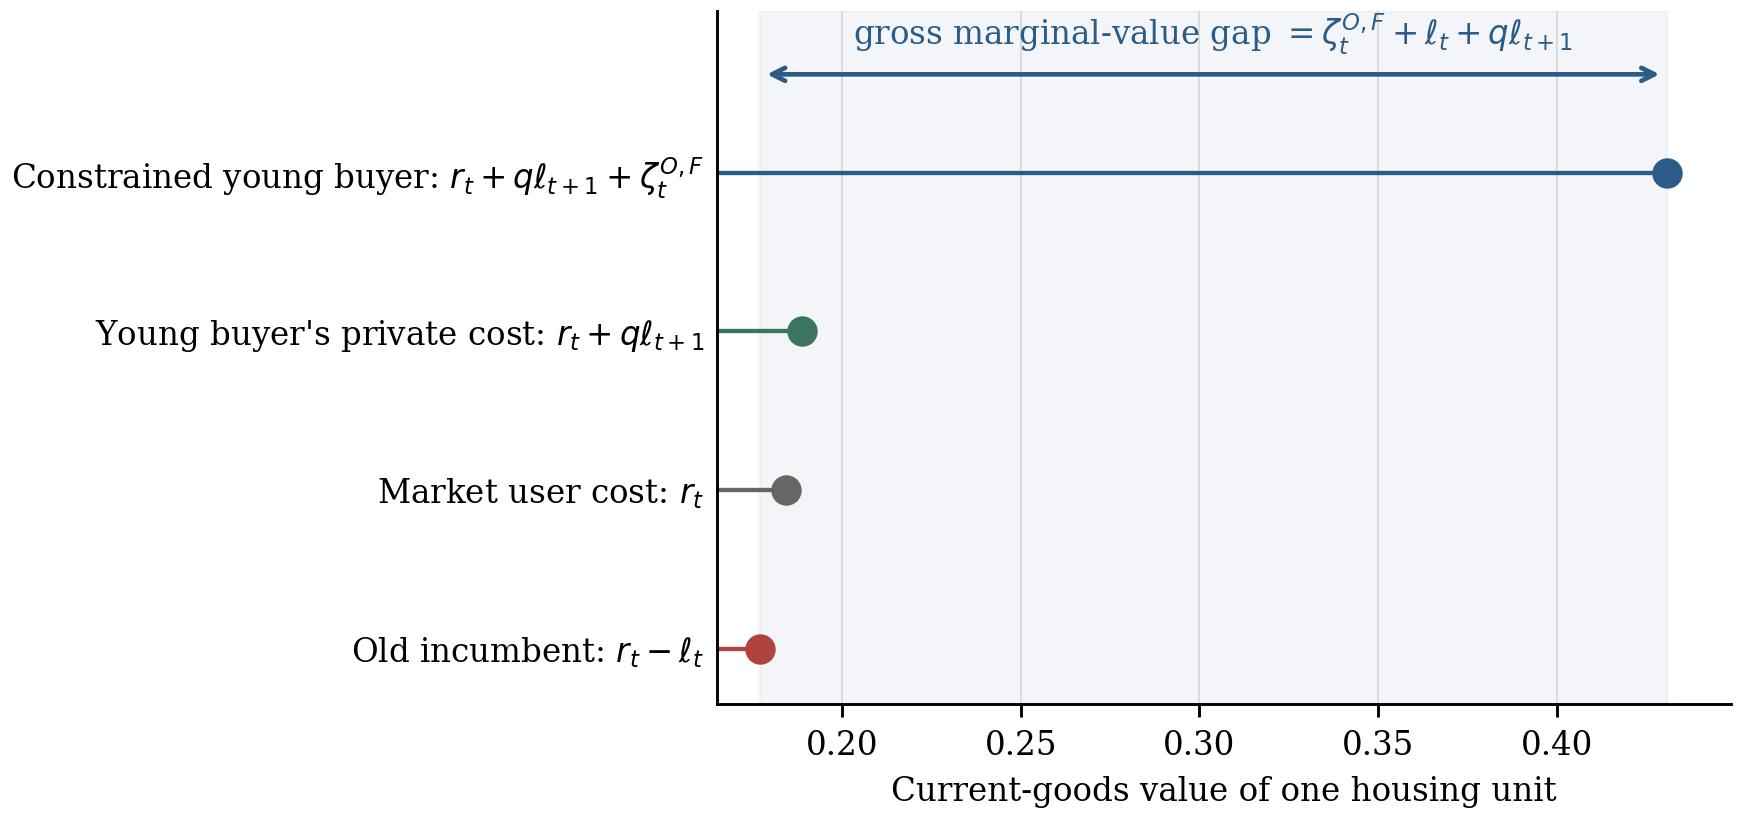
\includegraphics[width=0.88\textwidth]{figures/simplified_olg_reallocation_wedge.png}
\caption{Shadow-value decomposition on the computed path.  The financing wedge
raises the young buyer's value; realization taxes lower the old incumbent's
value and raise the buyer's anticipated private cost.  The displayed object is
the gross marginal-value gap.  Under the ledger in
Proposition~\ref{prop:olg_reallocation}, the reallocation is a Pareto
improvement for current households when this gap exceeds the real transfer
cost.}
\label{fig:olg_reallocation_wedge}
\end{figure}

\subsection{Housing access and fertility}
\label{app:olg_fertility}

Relaxing a binding housing limit has two effects.  It gives the family more
space, which makes children less costly, but it also requires the household to
pay for more housing, which leaves fewer goods for children.  The derivative
below compares these two forces.

Suppose $h=\widehat h$ binds and fertility remains interior.  Define
\begin{equation}
 x=\frac{\widetilde w_{it}^m-u_t^m\widehat h-\chi n}
 {1+k_{t+1}^m},\qquad
 s=\widehat h-\kappa n,
 \label{eq:olg_app_xs_binding}
\end{equation}
and collect the positive terms in
\begin{equation}
 \Delta=\frac{\vartheta_t}{n^2}
 +\frac{\chi^2}{(1+k_{t+1}^m)x^2}
 +\frac{\alpha\kappa^2}{s^2}>0.
 \label{eq:olg_app_fertility_delta}
\end{equation}
Implicit differentiation of the binding-fertility condition gives
\begin{equation}
 \frac{\dd n}{\dd\widehat h}
 =\frac{\alpha\kappa/s^2-\chi u_t^m/
 [(1+k_{t+1}^m)x^2]}{\Delta}.
 \label{eq:olg_fertility_derivative}
\end{equation}
On the interior old-age branch, the derivative is nonnegative exactly when
\begin{equation}
 \chi\leq
 \frac{(1+\beta A)\kappa(u_t^m+\zeta_{it}^m)^2}{\alpha u_t^m}.
 \label{eq:olg_fertility_sign}
\end{equation}

\begin{proof}[Derivation of \eqref{eq:olg_fertility_derivative} and
\eqref{eq:olg_fertility_sign}]
Let the left side of \eqref{eq:olg_binding_fertility} be
$F(n,\widehat h)$.  Direct differentiation gives
\begin{align}
 F_n&=-\Delta<0,\\
 F_{\widehat h}&=\frac{\alpha\kappa}{s^2}
 -\frac{\chi u_t^m}{(1+k_{t+1}^m)x^2}.
\end{align}
The implicit-function theorem gives
$\dd n/\dd\widehat h=-F_{\widehat h}/F_n$, which is
\eqref{eq:olg_fertility_derivative}.  Its numerator is the difference between
the space benefit and the goods-resource cost described above.  At a
constrained allocation,
\eqref{eq:olg_app_housing_kkt} implies
\begin{equation}
 \frac{x}{s}=\frac{u_t^m+\zeta_{it}^m}{\alpha}.
 \label{eq:olg_app_xs_ratio}
\end{equation}
Substituting this ratio into $F_{\widehat h}\geq0$ gives the condition in
\eqref{eq:olg_fertility_sign} on the interior old-age branch, where
$k_{t+1}^m=\beta A$.  On the capped old-renter branch the same derivation uses
$k_{t+1}^R=\beta(1+\omega_B)$.
\end{proof}

The same calculation separates two other partial-equilibrium channels:
\begin{equation}
 \frac{\partial n}{\partial\widetilde w_{it}^m}
 =\frac{\chi}{(1+k_{t+1}^m)x^2\Delta}>0,
 \qquad
 \frac{\partial n}{\partial u_t^m}
 =-\frac{\chi\widehat h}
 {(1+k_{t+1}^m)x^2\Delta}<0.
 \label{eq:olg_app_fertility_wealth_user_cost}
\end{equation}
At a fixed cap, more lifetime resources raise fertility and a higher housing
user cost lowers it.

A primitive sufficient condition, stronger than the exact condition, is
\begin{equation}
 \chi\leq\frac{(1+k_{t+1}^m)\kappa u_t^m}{\alpha},
 \label{eq:olg_app_fertility_sufficient}
\end{equation}
because $\zeta_{it}^m\geq0$.  When the down-payment constraint alone binds,
\begin{equation}
 \widehat h_{it}^O=\frac{b_i}{(1-\phi)P_t},\qquad
 \frac{\partial\widehat h^O}{\partial b_i}
 =\frac1{(1-\phi)P_t},\qquad
 \frac{\partial\widehat h^O}{\partial\phi}
 =\frac{b_i}{(1-\phi)^2P_t}.
 \label{eq:olg_app_cap_pass_through}
\end{equation}
The derivative with respect to $\phi$ isolates the cap-relaxation channel when
prices and resources are held fixed.  The two total derivatives on this branch
are
\begin{align}
 \frac{\partial n}{\partial\phi}
 &=\frac{\partial n}{\partial\widehat h}
 \frac{b_i}{(1-\phi)^2P_t},\\
 \frac{\partial n}{\partial b_i}
 &=\frac{\partial n}{\partial\widetilde w_{it}^O}
 +\frac{\partial n}{\partial\widehat h}
 \frac{1}{(1-\phi)P_t}.
 \label{eq:olg_app_financing_fertility_derivatives}
\end{align}
A change in liquid wealth has both a wealth channel and a housing-access
channel.  A funded policy additionally moves prices, transfers, and tenure,
and its aggregate response requires the equilibrium system.

\subsection{Mixed-tenure example}
\label{app:olg_computation}

The numerical example gives observed types common income and liquid wealth and
retains the logistic ownership preference in \eqref{eq:olg_owner_share}.  It
computes the two steady states and a terminally closed transition between them.
Table~\ref{tab:olg_app_parameters} lists the parameters.

\begin{table}[!htb]
\centering
\caption{Parameters of the mixed-tenure construction}
\label{tab:olg_app_parameters}
\footnotesize
\begin{tabular}{@{}llr@{\qquad}llr@{}}
\toprule
Object & Parameter & Value & Object & Parameter & Value\\
\midrule
Bond price & $q$ & 0.50 & Mortgage share & $\phi$ & 0.80\\
Property tax & $\tau^p$ & 0.05 & Gains-tax rate & $\tau^g$ & 0.20\\
Space weight & $\alpha$ & 0.40 & Space per child & $\kappa$ & 0.50\\
Goods per child & $\chi$ & 0.15 & Young discount & $\beta$ & 0.40\\
Old housing weight & $\gamma$ & 0.30 & Estate weight & $\omega_B$ & 0.40\\
Income & $y$ & 1.00 & Liquid wealth & $b$ & 0.06\\
Household formation & $\nu$ & 2.00 & Housing stock & $\bar H$ & 2.00\\
Rental limit & $h_R^{\max}$ & 0.45 & Owner limit & $h_O^{\max}$ & 2.00\\
Owner intercept & $\bar\xi$ & $-0.15$ & Taste scale & $\sigma_\xi$ & 0.12\\
\bottomrule
\end{tabular}
\end{table}

At date zero, $\vartheta$ rises permanently from $0.35$ to $0.50$.  Solving
\eqref{eq:olg_steady_state_system} gives Table~\ref{tab:olg_app_steady_states}.

\begin{table}[!htb]
\centering
\caption{Positive steady-state endpoints}
\label{tab:olg_app_steady_states}
\footnotesize
\begin{tabular}{@{}lrr@{}}
\toprule
Object & Initial steady state & Final steady state\\
\midrule
Fertility preference $\vartheta$ & 0.3500 & 0.5000\\
Average fertility $\bar n$ & 0.5000 & 0.5000\\
House price $P$ & 0.3427 & 0.4844\\
Per-household transfer $T$ & 0.00589 & 0.00602\\
Young owner share & 0.7486 & 0.5149\\
Renter fertility & 0.3527 & 0.4368\\
Owner fertility & 0.5495 & 0.5596\\
Young renter housing & 0.4500 & 0.4500\\
Young owner housing & 0.8754 & 0.6193\\
Old renter housing & 0.4500 & 0.4500\\
Old owner housing & 0.6582 & 0.4649\\
Young and old cohort mass & 1.4553 & 2.0103\\
\bottomrule
\end{tabular}
\end{table}

Average fertility is $1/\nu=0.5$ at both endpoints, but conditional fertility,
tenure, housing, prices, and population scale differ.  Both roots are locally
regular: the Jacobian determinants in $(\log P,\log T)$ are $-0.00466$ and
$-0.00433$.

On impact, average fertility rises to $0.6223$ and the young cohort expands one
period later.  The price rises from $0.3427$ to $0.3800$, reaches $0.4975$ at
date 3, and then approaches $0.4844$.  Gains taxes are positive on dates 0--3
and 7--8.  Thus one preference change generates taxable gains for several
cohorts even though gains are zero in both steady states.

Both tenures have positive mass.  The young renter and owner housing limits
bind, and the owner's limit is financial.  The old rental limit binds, while
old owners are interior.  The maximum scaled equilibrium residual is
$6.51\times10^{-10}$; extending the horizon from 28 to 32 changes the first
twenty dates by at most $3.11\times10^{-15}$.

The steady-state existence conditions are also satisfied on the declared
price--transfer grid: the fiscal map is a contraction and the replacement
residual changes sign at the two price boundaries.


\clearpage
\bibliographystyle{plainnat}
\bibliography{references,main_bib,lit_review_extra}

\end{document}
